%% LyX 1.5.5 created this file.  For more info, see http://www.lyx.org/.
%% Do not edit unless you really know what you are doing.
\documentclass[12pt,english]{report}
\usepackage[T1]{fontenc}
\usepackage[latin9]{inputenc}
\setcounter{secnumdepth}{3}
\setcounter{tocdepth}{3}
\usepackage{float}
\usepackage{graphicx}
\usepackage{setspace}
\onehalfspacing

\makeatletter

%%%%%%%%%%%%%%%%%%%%%%%%%%%%%% LyX specific LaTeX commands.
%% Because html converters don't know tabularnewline
\providecommand{\tabularnewline}{\\}
\floatstyle{ruled}
\newfloat{algorithm}{tbp}{loa}
\floatname{algorithm}{Algorithm}

\makeatother

\usepackage{babel}

\begin{document}
\pagestyle{empty}
\newpage
\begin{center}
\begin{LARGE}
Fast User-level Inter-thread Communication, Synchronisation and Streaming
\end{LARGE}
\end{center}
\vspace{1in}
\begin{center}

\includegraphics[scale=0.3]{uom}
\end{center}
\begin{center} 
\begin{large} A thesis submitted in partial fulfilment of the requirements for the degree of Bachelor of Science (Hons)
\end{large}
\end{center}
\begin{center} 
\begin{large}University of Malta \\ Department of Computer Science
\end{large}
\end{center}
\vspace{2in}
\begin{center}
\begin{large} By \\ Li Lin \\ May 2008\end{large}
\end{center}

\newpage 
\pagestyle{plain}
\pagenumbering{roman} 
\setcounter{page}{1}
\begin{abstract}
Since 2000, the fast user-level thread scheduler SMASH has been actively developed at the University of Malta. This project's objective is to design and implement several user-level inter-thread communication constructs for SMASH. Since communication and synchronization among threads in a process is heavily used in most multi-threading programs, the efficiency of inter-thread communications affects the efficiency of the whole program. In the past, those communication and synchronization constructs were built with locks, but this lock-based approach has some problems such as potential deadlock(or livelock), starvation and priority inversion. In order to solve these problems, lock-free algorithms were invented. A concurrent algorithm is lock-free, if after a finite step of execution, at least one of the participating threads is guaranteed to progress. Recently there is a lot of interest in lock-free algorithms in the research community. In this project, all the inter-thread communication constructs considered have two implementations: the lock-based implementation and the lock-free implementation. The performance of concurrent programs using these user-level constructs is measured and compared with the performance of programs using kernel-level inter-thread communication constructs. Besides, the differences between the lock-based implementations and lock-free implementations are also analyzed.
\end{abstract}
\section*{Acknowledgments}
I would like to experss my gratitude to my supervisor Dr. Kevin Vella who guided me to the final goal. It was his knowledge and patience that enabled me to complete this proejct successfully. During this project, Mr. Alan Casar helped me a lot so that I was able to understand SMASH in a very short time and Mr. Reggie Cushing gave me a lot of help in the hardware issues. So I would also like to give my thank to them for their assistance.
\tableofcontents{}
\listof{algorithm}{List of Algorithms}
\listoffigures
\newpage 
\pagestyle{plain}
\pagenumbering{arabic} 
\setcounter{page}{1}


\chapter{Introduction}

SMASH\cite{16} is a user-level thread system running on top of Linux.
Originally, it was developed by Kurt Debattista in 2001 on Linux 2.2
series kernels. Since then it has been actively developed at the University
of Malta by several students. By the time of this writing, a lot of
work has been done. Now it runs on Linux 2.6 series kernels and has
six different implementations. However, it still lacks user-level
inter-thread communication and synchronization constructs such as
mutexes, semaphores, etc. The only inter-thread communication construct
it has is the simple communication channel. The main objective of
this final year project is to implement a inter-thread communication
library for a particular implementation of SMASH, and to find out
how these constructs affect the performance of the SMASH system. Since
these constructs are shared objects among threads, to guarantee the
consistency of these objects, certain synchronization mechanisms have
to be used. When implementing these synchronization algorithms, there
are two approaches: the lock-based approach and the lock-free approach.
In lock-based algorithms, critical sections are protected by some
forms of locks. A typical example is the spin lock, which is widely
used on SMP systems\cite{5}. In this project, all lock-based designs
use spin locks. Lock-free algorithms are also exploited. Although
lock-free and wait-free algorithms have drawn a lot of attention in
the last decade, they are not heavily used in thread scheduling and
inter-thread communications, instead, a lot of effort was made to
develop general lock-free and wait-free ADTs. In this project, all
user-level inter-thread communication constructs have their corresponding
lock-free or wait-free implementations. 

Lock-based algorithms are relatively easier to design, in the simplest
case, one can just use a spin lock to surround the entire execution
of the algorithm to guarantee its atomicity. However, this approach
usually introduces extra overhead because a thread may have to wait
even if the thread executing the algorithm is in the entry section
or exit section, so for efficiency sake, the granularity of critical
sections should be kept small. The extreme case is the lock-free algorithm,
in which the size of critical sections are reduced to just single
atomic instructions. The drawback of this approach is that fine-grained
algorithms are difficult to design, and also difficult to reason with. 


\section{The structure of this documentation}

In Chapter 2, background knowledge about SMP systems, lock-free algorithms,
processes and threads is given, then Chapter 3 gives a literature
review on interprocess communication constructs on different systems.
In this chapter, two kinds of operating systems are mentioned: systems
with monolithic kernels and ones with microkernels. In Chapter 4,
we will discuss the implementation of the inter-thread communication
constructs for SMASH. Results for the performance of these constructs
are given and discussed in Chapter 5.


\chapter{Background}


\section{SMP systems}

Symmetric Multiprocessing\cite{5} is a computer architecture in which
a set of identical CPUs are connected together though a shared memory
bus so that they can co-operate to get more computational power. Each
CPU has its own caches and registers, but the main memory of the system
is shared amongst all CPUs and access to the main memory is uniform,
i.e. the access time to a memory location is the same for all CPUs
in the system, this model is called Uniform Memory Access(UMA)\cite{5}.%
\begin{figure}


\caption{Architecture of SMP}


~~~~~~~~~~~~~~~~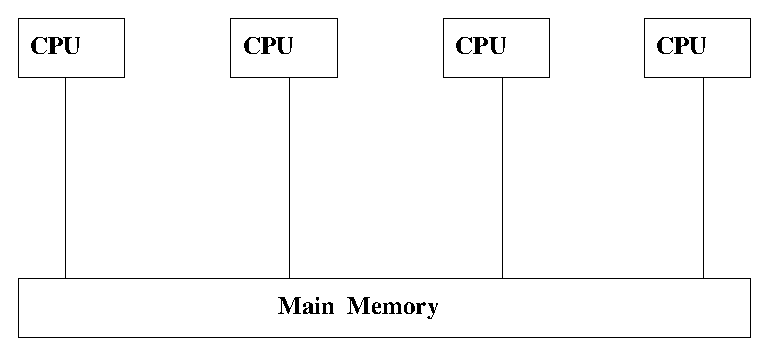
\includegraphics[scale=0.7]{SMP_arch}


\end{figure}
 Another memory model is the Non-Uniform Memory Access model, in which
CPUs have their own memory and each CPU can access other CPU's local
memory, but in that case, the access is relatively slow. In order
to utilize this architecture, a program has to be subdivided into
several parts that can be processed independently, so that these parts
can be executed on different CPUs concurrently. 


\section{Synchronization support}

On SMP systems, different CPUs usually have to access some shared
data concurrently. In order to guarantee the consistency of the shared
data, we need some kind of synchronization mechanisms. Modern architectures
offer some atomic instructions which allow us to implement those high-level
synchronization algorithms. We list some of these atomic instructions.


\subsection*{Test\_And\_Set}

This instruction atomically check whether the value stored in a memory
location is true or not. If the value is false, then it changes the
value to true, otherwise it does nothing. %
\begin{algorithm}[h]
\caption{Pseudo code for \emph{Test\_And\_Set}}


TestAndSet(var) \{

~~~if(var == false)

~~~~~var = true;

~~~~~return true;

~~~else 

~~~~~return false;

\}
\end{algorithm}



\subsection*{Fetch\_And\_Add}

This instruction reads the value from a given memory location and
increments the value in that location by a number given by the user.
%
\begin{algorithm}
\caption{Pseudo code for \emph{Fetch\_And\_Add}}


FetchAndAdd(void {*} location, int num) \{

~~~int old = {*}location

~~~{*}location = {*}location + num

~~~return old

\}


\end{algorithm}



\subsection*{Swap}

The \emph{Swap }atomically exchanges the values stored in two memory
places, these places can be locations in the main memory or registers.
A typical implementation is given by Algorithm\emph{ }\ref{alg:Swap},
but in our case, we slightly modify the implementation for convenience's
sake. Our implementation is given by Algorithm\emph{ }\ref{alg:The-semantics-of}.
%
\begin{algorithm}
\caption{\emph{\label{alg:Swap}Swap}}


Swap(void {*} location1, void {*} location2) \{

~~~tmp\_value = {*}location1

~~~{*}location1 = {*}location2

~~~{*}location2 = tmp\_value

\}


\end{algorithm}
%
\begin{algorithm}
\caption{\label{alg:The-semantics-of}The semantics of our implementation for
swap}


long swap(long {*} location, long value) \{

~~~long tmp\_value = {*}location

~~~{*}location = value

~~~return tmp\_value

\}


\end{algorithm}



\subsection*{Compare\_And\_Swap}

\emph{Compare\_and\_Swap} works in the way as Algorithm\emph{ }\ref{alg:Pseudo-code-for}
shown: it compares the content of a given memory location with its
old value which is read some time before, if the content is the same
as the old value, then it writes the new value to the memory and returns
TRUE, otherwise, it does nothing to that memory and returns FALSE.
The whole process is atomic.%
\begin{algorithm}[H]
\caption{\label{alg:Pseudo-code-for}Pseudo code for \emph{Compare\_and\_Swap}}


bool CAS(Location, old, new) 

~~~~if (location == old)

~~~~~~location=new

~~~~~~return true

~~~~else return false
\end{algorithm}
According to \cite{20}, \emph{Compare\_And\_Swap} was first implemented
in the IBM System 370, and now it is widely supported on many architectures,
for example x86-32, x86-64, Sun Sparc etc.


\subsection*{Linked-Load/Store-Conditional(\emph{LL/SC})}

\emph{LL/SC} works as follows: the instruction \emph{LL} first reads
the content from a memory location, then \emph{SC} can be used to
update the memory location. If the content of that memory has not
been changed, then the new value is stored into the memory and \emph{SC}
returns \emph{TRUE}. Otherwise the memory is not updated and \emph{SC}
returns \emph{FALSE}. However, in practice, no architectures that
support \emph{LL/SC} such as Alpha, MIPS, PowerPC, etc, implement
the full semantics of \emph{LL/SC} in hardware in the sense that memory
accesses inbetween \emph{LL} and \emph{SC} is restricted, for example
none of these architectures allow nesting or interleaving of \emph{LL/SC}
pairs. Besides, on some platforms, context switches, another \emph{LL}
operation or even another \emph{load} or \emph{write} operations may
cause \emph{LL/SC} to fail spuriously. This instruction is available
on systems like MIPS and PowerPC.


\section{Spin locks}

On uniprocessor systems, an execution sequence can be combined together
so that it is not interruptable by disabling the interrupt of the
CPU at the beginning of the sequence and re-enabling the interrupt
at the end. However, this mechanism is not valid on SMP systems, because
we can only disable the interrupts on some CPU locally, other CPUs
can still access the critical section. In this case, spin locks are
used to protect critical sections. A spin lock can take one of two
values: the integer 1 to denote the lock is locked, 0 to denote it
is free. When the spin lock is 1, other CPUs trying to obtain the
lock just keep looping until it is released. Algorithm \ref{alg:Pseudo-code-of}
gives the pseudo code.

%
\begin{algorithm}[H]
\caption{\label{alg:Pseudo-code-of}Pseudo code of Spin locks}


L1~~~~getSpinlock(int lock) \{

L2~~~~~~~while(lock == 1);

L3~~~~~~~lock = 1;

L4~~~~\}\\


L5~~~~releaseSpinlock(int lock) \{

L6~~~~~~~lock = 0;

L7~~~~\}
\end{algorithm}


However, to implement the above semantics, special atomic instructions
are needed, because there is a danger between L2 and L3. When the
lock is released at L2 and before it is locked again by another thread
at L3, it is possible that more than one thread has finished L2, and
as a result, more than one thread will enter the critical section.
Hence, we need an instruction to implement L2 and L3 atomically. \emph{Test\_and\_Set}
is this kind of instruction. It tests whether the content of a shared
variable is true or not, if false, it sets the variable to true, otherwise
it does nothing. The entire process is done atomically. Then spin
locks can be implemented properly with it.

%
\begin{algorithm}
\caption{Proper implementation for spin locks}


getSpinlock(int {*} lock) \{

~~~while(TestAndSet(lock));

\}

releaseSpinlock(int {*} lock) \{

~~~{*}lock = 0;

\}


\end{algorithm}


Although the above implementation is correct, it has another problem.
When multiple threads are trying obtain the spin lock, the memory
where the lock is stored becomes a hot-spot, because all threads keep
accessing it. In this case, we will have high memory contention. In
order to avoid this problem, we can use \emph{Test\_Test\_and\_Set,}
the basic idea is that a thread uses \emph{Test\_And\_Set} to change
the value of the spin lock, if it has been locked by another thread,
instead of spinning on the variable directly, it spins on a local
copy of the lock in its local cache, when the lock is released, those
copies stored in CPU's local cache will be invalidated automatically
by the cache coherence mechanism, CPUs will re-read the value of the
lock into their local cache. In the way, the waiting threads do not
access the memory during spin-waiting, instead, they just access the
copy in the local CPU cache, hence the memory contention is reduced.%
\begin{algorithm}
\caption{Spin lock with \emph{Test\_Test\_And\_Set}}


getSpinlock(int {*} lock) \{

~~~while({*}lock);

~~~while(TestAndSet(lock));

~~~~~~while({*}lock);

\}

releaseSpinlock(int {*} lock) \{

~~~{*}lock = 0;

\}


\end{algorithm}


Another problem of spin locks is that it is unfair, i.e. some threads
may be delayed for a long time even they come earlier. Because there
is no ordering among those waiting threads, they just spin-wait for
the lock to be freed. It is nondeterministic that who will get the
lock. This will cause high latency on some threads. The MCS-lock\cite{13}
solves this problem by enforcing a FIFO ordering. Linux developers
used another algorithm called \emph{ticket spin lock} to provide the
FIFO ordering for spin locks. This algorithm is an adoption of the
\emph{Ticket algorithm}\cite{6,17}\emph{.} On a system with a small
number of CPUs, the ticket spin lock performs better, because it is
less complicated, but it still suffers from the memory contention
problem. On the other hand, The MCS-lock performs better in a system
with a large number of CPUs, because it utilizes the local cache of
each CPU. A CPU just spin-waits on a variable stored in its local
cache, hence the contention caused by busy-waiting is avoided.


\section{Lock-free algorithms}

There are some problems with lock-based algorithms. First, there are
potential dead(or live) locks. A dead lock is a situation in which
all thread wait for one another cyclically, but no one is in the critical
section. As a result, they all wait forever, if they are busy-waiting,
then we call it a live lock. Second, priority inversion happens when
a high priority thread tries to acquire the lock which is currently
held by a low priority thread, so the former one has to wait until
the latter releases the lock. This may cause serious problem on real-time
systems. The third problem is convoy effect. 

To overcome these problems, lock-free algorithms are used. A concurrent
algorithm is lock-free if after a finite number of execution steps,
at least one of the participating threads progresses to the final
goal. Lock-free algorithms are free of dead locks, but some particular
threads may be delayed indefinitely. A stronger concept is the wait-free
algorithms. An algorithm is wait-free if after a finite number of
steps, all participating threads can finish.

Normally, wait-free algorithms are more efficient, however, they are
hard to find. Currently most of wait-free algorithms are based on
some strong assumptions such as fixing number of participating threads
before the execution. Hence they are quite restricted.

Implementing these lock-free algorithms also needs some special atomic
instruction supported by the hardware. The most commonly used instructions
are \emph{Compare\_and\_Swap}, and \emph{Link-Load/Store-Conditional.
}Herlihy\cite{25} has proved that both \emph{CAS} and \emph{LL/SC}
are powerful enough to construct most lock free data structures shared
by more than two threads but \emph{Fetch\_And\_Add}, \emph{Test\_And\_Set}
and \emph{Swap} are not. And even some more sophisticated atomic structures
like atomic stack operations are not enough, which is quite surprising
because these operations are quite powerful. In \cite{19}, a software
level lock-free \emph{LL/SC} with full semantics was implemented with
\emph{CAS} provided by the hardware.


\subsection{ABA problem}

When implementing lock free data structures by using \emph{CAS}, one
critical issue is the ABA problem. It is described as follows: Suppose
a thread \emph{A} reads data from a memory location \emph{l}, then
tries to update the content of \emph{l} by using \emph{CAS}. But after
\emph{A} has read the value and before the update happens, another
thread \emph{B} first changed the content of \emph{l} then changed
it back to its original value. Then when \emph{A} tries to update
the content of \emph{l} by using \emph{CAS}, it will success without
noticing what \emph{B} has done. This problem was first identified
on the IBM System 370\cite{7} and may lead to data corruption. \emph{LL/SC}
would not suffer from this problem if its full semantics were implemented.
However, due to practical reasons, no hardware has ever implemented
\emph{LL/SC} with its full semantics, so existing implementations
of\emph{ LL/SC} also has this problem. The most efficient way to solve
the ABA problem is to use \emph{CAS2}(or Double Compare\_And\_Swap),
which is basic the same as \emph{CAS} but keeps a count of the number
of times a memory location is modified, hence solving the ABA problem.

%
\begin{algorithm}[h]
\caption{Pseudo code for \emph{CAS2}}


boolean CAS2(var,count,old-value,old-count,new-value) \{

~~~~~if(var == old-value AND count == old-count)

~~~~~~~~var = new-value;

~~~~~~~~count++;

~~~~~~~~return TRUE;

~~~~~else return FALSE;

\}


\end{algorithm}


On 32-bit machines, \emph{CAS2} operates on 8 bytes atomically so
that users can use 4 bytes as data to be updated and the other 4 bytes
as the update counter. However, on some 64bit machines, to implement
\emph{CAS2}, one needs atomic machine code instructions that operate
on 16 bytes which are not available on these CPUs, hence this technique
can not be applied in such cases.

A second solution is to use hazard pointers designed by Michael\cite{1,19,20}.
The basic idea of this approach is that each thread holds a set of
one-writer multiple-reader pointers called hazard pointers. Only the
owner thread can write to them, others can only read them. When a
thread accesses a memory location, it makes one of its hazard pointers
point to that location. When a thread tries to recycle the memory,
it searches all hazard pointers owned by other threads to check whether
some threads are still using the memory, and the memory will not be
recycled until no threads use it any more. In this way, the ABA problem
is avoided.

The third way is to use some lock-free reference counting algorithms
for example, Valois' lock-free reference counting algorithm\cite{12}.
The core idea is that each piece of memory participating in the lock-free
data structure contains a counter, and any thread referencing the
memory location will increment the counter. After use, the counter
will be decremented and the memory will not be recycled until the
counter is zero. 


\subsection{Lock-free First In First Out queues}

In this project, the most commonly used data structures are First
In First Out queues. They are used as message queues and waiting queues
for semaphores and mutexes. Michael and Scott developed a lock-free
FIFO queue\cite{18}, which Debtattista used in one of the SMASH implementations.
However, he showed that its performance was not as good as expected,
and suggested in \cite{16} that the main problems may be the memory
management and the extensive use of the \emph{CAS} instruction which
is relatively costly. There are many other lock free FIFO queue designs
which trying to improve the performance. We used a design from \cite{2},
which by experiments\cite{2} is almost twice faster than MS-queue
in most cases. Another problem that causes performance degradation
is that \emph{CAS},\emph{ LL/SC} and \emph{CAS2} are costly, and they
are used intensively in enqueue- and dequeue-operations. In fact,
for most cases, the use of these expensive instructions are redundant,
since errors rarely happen, hence some work has been done to try to
reduce the frequency of use of these instructions. Some notable works
are \cite{3} and \cite{24}, in which developers implemented a lock-free
FIFO queue as a double-linked list and only one \emph{CAS} is used
in the enqueue operation, whenever an error is detected, an auxiliary
function is used to fix it. Although the error-fixing is complicated
and more expensive than \emph{CAS}, the queue still performs much
better than those queues which require intensive use of \emph{CAS}.
So far we have not found any linked list-based wait-free FIFO queues
for a scheduler like SMASH. There are some wait-free FIFO queues available,
but they are either array-based or else they depend on special scheduling
policies.


\section{Processes, kernel and user-level threads}

Multitasking plays a critical role in most general purpose operating
systems. At first, Unix systems implemented multitasking by using
the concept of processes. A process is a running instance of a program
which has its own set of resources such as address spaces, registers,
open file descriptors and so on. The system creates multiple processes
then schedules among them so that users get the impression that multiple
programs are running concurrently. The main problem of this approach
is that the context switch between two processes is very expensive.
To switch from a process to another, the system has to do a lot of
tasks like switching from user mode to kernel mode, saving the current
registers used by the process and changing the address space because
each process has its own virtual memory space. In addition, communications
between processes is also expensive, because messages have to be copied
from the address space of one process to that of another process,
although there are techniques like Shared Memory and COW(Copy On Write)\cite{31}
that can be used to reduce this kind of overhead, in many cases, message
copying is still necessary. Besides, inter-process communication usually
implies context switches between processes, which are costly in their
own right. To overcome this problem, the concept of a thread or LWP
(Light Weight Process) was introduced. Threads within a process can
be scheduled by the system just like the system schedules processes,
but they share a lot of resources, for example, threads within a process
have no private address space, therefore context switches between
threads are cheaper. Also communications between threads are cheaper
and easier to implement due to the fact that threads share a single
address space. 

There are two kind of threads: kernel threads and user level threads.
Kernel threads are implemented in the kernel, i.e. when such a thread
is created, the kernel maintains all kind of information about it.
This kind of threads is normally preemptive. However, the context
switch is a bit expensive, because the information about a thread
is maintained by the kernel, to do the context switch, the program
has to switch from user mode to kernel mode and save the current status
of the thread execution like content of registers, program counter,
stack pointer into the data structure representing the thread, but
switching from user mode to kernel mode is expensive. In addition,
to preempt a running thread, the content of all registers has to be
saved because we do not know which registers are currently being used
by the thread, and this operation is particularly expensive on RISC
CPUs since they normally have a large set of registers. In some systems
like Mach\cite{26,29,31} and Windows, the notion of processes is
quite different from the traditional one from UNIX, as processes in
these systems are just running contexts or environments in which kernel
threads run. For example in the Mach system, once a process, which
are also named \emph{tasks }in Mach, is created, the system has to
create a so called main thread in the process.

User level threads, as the name suggests, are threads implemented
in user space, the kernel has no information about them, hence they
are non-preemptive, but cooperative. Hence, a running thread has to
release the CPU explicitly so that other user-level thread can run.
The advantage is that the system is able to know that what registers
are being used by the thread, therefore only a subset of registers
need to be saved. Hence, user level threads are normally faster than
kernel level threads. In fact, SMASH\cite{16} applied this technique
and reduced the time of context switch to roughly \emph{28ns}\cite{16}\emph{.}
Another advantage of user-level thread is that the scheduler also
runs in user space, hence scheduling between threads does not need
to go from user mode to kernel mode. There are many implementations
of user level threads, for example Mach's cthreads\cite{26,31}, pthreads
on early versions of FreeBSD and SMASH.


\subsection{SMASH}

SMASH\cite{16} is a user level thread system. It uses the two-level
thread scheduling model.%
\begin{figure}
\caption{Two Level thread scheduling}


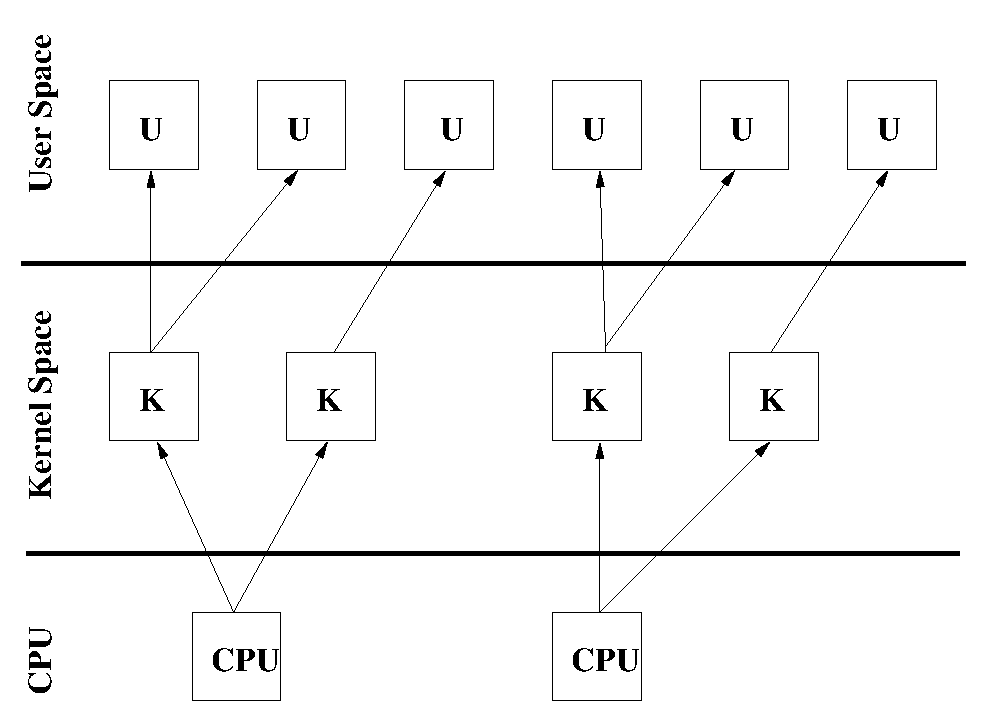
\includegraphics{two-level-scheduling}


\end{figure}
 The basic idea is to create a set of user level threads on top of
different kernel threads. The main advantage of this approach is that
when a user-level thread is blocked for some reasons, other user-level
threads on top of different kernel threads can still run. SMASH is
partially based on another user-level thread scheduler called MESH
developed by Boosten\cite{22,23} and SMP-MESH developed by Cordina\cite{11},
it is actively being developed in the university of Malta. In 2000,
Based on MESH, Joseph Cordina developed SMP-MESH as his Final Year
Project, his implementation of SMP-MESH used a shared run queue which
is protected by spin locks. Then in 2001, Debattista wrote SMASH based
on Cordina's work as his master degree. He designed the uniprocessor
version of SMASH and the SMP versions. He came up with six different
designs for the SMP version of SMASH, which can be categorized into
two main categories: SMASH with shared run queue and SMASH with per-CPU-run-queue.
SMASH runs on both uniprocessor and SMP machines, the internal implementations
are quite different, the uniprocessor version is purely cooperative,
in a running SMASH instance, there is only one thread scheduler running
in the user space and all SMASH threads are scheduled by it. A thread
has to yield the CPU explicitly so that other threads can run. On
the other hand, the SMP version take the benefit of multi-CPUs, it
creates one thread scheduler running on top of a kernel thread for
each CPU. SMASH threads on the same CPU are cooperative, however,
on the whole system they are preemptive, i.e. if SMASH threads on
different CPUs are accessing some shared data, some of them may be
preempted by the underlying kernel threads. For efficiency sake, kernel
threads on which the SMASH schedulers run are bounded to the corresponding
CPUs, hence even one of these kernel threads is scheduled by the kernel
thread scheduler, it will be woken up on the same CPU. On Linux 2.2
series kernels, this kind of operation was not supported, so Debattista
had to apply a patch to the Linux kernel he used, from Linux kernel
2.4 onwards, this operation can be done by a system call named \emph{sched\_setaffinity()},
so Reggie Cushing patched SMASH so that it can run on Linux 2.4 systems,
and then Alan Casar further patched it so that SMASH can run on Linux
2.6. 

In this project, we used a SMASH implementation with shared run queue
with fine-grained locks on a SMP system. With this implementation,
we have one thread scheduler per processor running on top of a kernel
thread. There is a single shared run queue among them. The run queue
is implemented with Michael and Scott dual-lock FIFO queue\cite{18}.
Each scheduler will pick up a user-level thread from the shared run
queue and run it. When a thread yields the CPU, it first saves the
current context, then the thread is re-inserted onto the run queue.
If the run queue is empty and one of the SMASH scheduler has no thread
to run, then the underlying kernel thread on which the SMASH scheduler
runs will sleep on a system semaphore, and it is woken up when a new
job arrives. %
\begin{figure}
\caption{The architecture of SMASH with shared run queue(from \cite{14})}


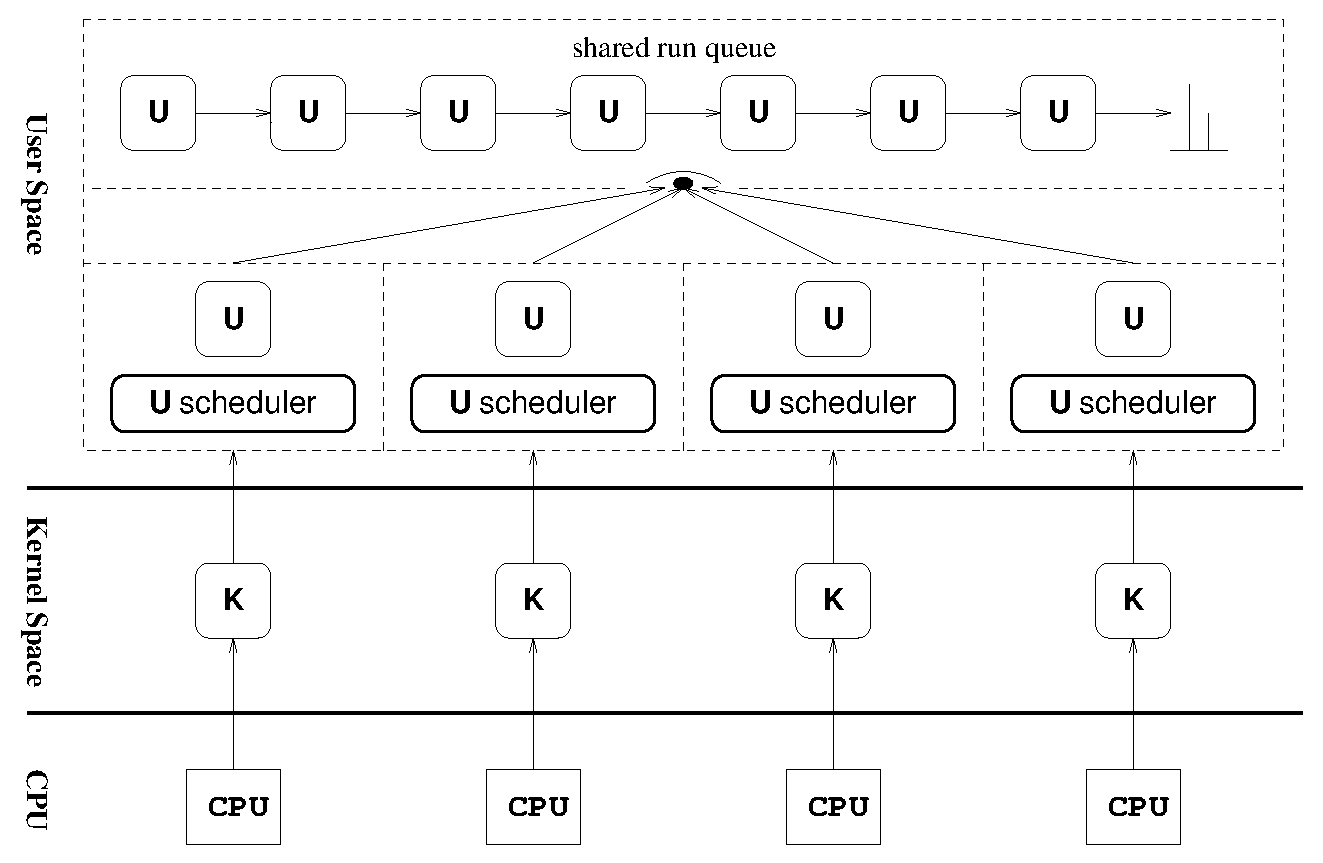
\includegraphics[scale=0.7]{shared}


\end{figure}



\chapter{Interprocess communication and synchronization constructs}

In modern operating systems such as UNIX and Windows, inter-process
communications play a crucial role since they are intensively used.
In this chapter, we are going to give an overview on these constructs. 


\section{System V IPC}

System V \cite{31}is one of the major branches of UNIX systems\cite{31}.
It provides three kinds of interprocess communication constructs:
semaphore, message queue and shared memory. These constructs are called
System V IPC and influence heavily other UNIX/UNIX-like systems. BSD
systems and Linux also implement these constructs.


\subsection{Semaphores}

Semaphores are described in \cite{26,31}. They contain a integer
counter and support two atomic operations \emph{signal} and \emph{wait}.
The signal operation decrements the counter of the semaphore. If the
result is non-negative, then the process continues its execution,
otherwise, it blocks until other processes wake it up with the \emph{wait
}operation. The \emph{signal} operation increments the counter and
checks if there are any processes waiting for the semaphore. If so,
it will wake one waiting process up.

Semaphores are used to provide some synchronization mechanisms among
processes. One application is that they can be used to limit the number
of processes accessing a shared resource, for example, a web server
can use semaphores to control the number of clients accessing a particular
page. Another important use is that when a semaphore is initialized
to 1, it can be used to provide mutual exclusion to a critical section,
in this case, only one process is able to access the shared resource,
and other processes have to wait. 

The semaphore is a very important interprocess communication construct
and is widely used in concurrent programming. Semaphores are high
level constructs, they are shared objects on their own, and to implement
semaphores, one needs low level synchronization constructs like spin
locks. In fact, on Linux systems, system V semaphores are implemented
in the kernel with spin locks, and on Linux systems, operations on
semaphores always enter the kernel, operate on the semaphore and then
return to the user space even if there is no contention on the semaphore,
which is quite expensive. 


\subsection{Message queues}

A message queue\cite{21,31} is implemented as a linked list of individual
messages located in the kernel. A message has a integer field as its
type and a message body containing the actual data. To send a message
to a message queue, a process has to hold the appropriate permissions,
and the message is copied from the sender to the queue in the kernel,
if the queue is full or the message is too large, then the process
either blocks until the required space is available or it gets an
error immediately. To receive messages from a message queue, a process
also have the corresponding permissions. And the entire queue is searched
for the specified type of messages, the first one found will be copied
from the queue to the located that is pre-defined then the message
is removed from the queue. If no such messages are found, then the
receiver can choose either blocks or returns immediately. 


\section{Mach's IPCs}

Traditionally, kernels of operating systems are monolithic, their
components are highly coupled together and runs in kernel mode. The
advantage of this approach is that it is very efficient, but as the
kernel grows larger, it suffers from problem such as security and
maintainability. Hence developers tried to move some functionality
out of the kernel and to implement them as independent processes running
in user mode, the kernel only provides some very basic services such
as address spaces and IPCs, and the components communicate and cooperate
with each other though interprocess communication constructs. Therefore,
the efficiency of the interprocess communication is very crucial on
such systems since they are heavily used. Mach\cite{29,31} is such
a microkernel implementation. 

In Mach, only a very few components such as device drivers, task scheduler,
etc, are implemented in the kernel, other components like Pager, File
systems, etc are implemented in user space. All these components communicate
with each other though ports. A port is an unidirectional bounded
message queue in the kernel. Mach ensures security by the concept
of \emph{rights. }A right has two parts: a port name and a capability
on that port. There are two kinds of capabilities on a port: \emph{send}
which allows a process/thread send messages to a port, or \emph{receive}
which allows a process/thread receive messages from a port. For a
given port, only one process can hold its \emph{receive} capability,
but there can be many processes/threads have the \emph{send} capability
on it. Since a port is a bounded queue, if a process tries to send
a message to a port when it is full, the process either aborts immediately
or it blocks until there is a space available in the queue. 

A message has a fixed-length header and a variable-length message
body. A message header contains information such as the destination
port, the length of the message body, etc. A message body consists
of different data sections, each section has its own type. In the
past, messages are always copied from the sender to the receiver,
but this is quite expensive when the message is large, therefore,
from Mach 2.5, a technique called Copy On Write(COW) was used. With
this technique, instead of copying the message, a sender just sends
the pointer to the message body to the receiver, if the receiver just
reads the message and does not modify it, no copy operation will happen
at all. Of course, the details is more complicated and in reality,
this is done though the virtual memory system.


\section{L4's IPCs}

Mach was categorized as the first-generation microkernel, one of its
critical problems is that its interprocess communications are too
slow\cite{14}. It was generally believed that it was the overhead
caused by things like vertical switches, address space switches and
memory penalties that made the IPC slow. However, later researches
\cite{8,9}show that these kinds of overheads can be largely reduced
by a proper kernel design. L4 family\cite{8,9} is a typical example
of the second generation microkernels. It was developed at GMD in
1995. In the kernel, it only implements only three components: address
spaces, threads and interprocess communication. 

L4's IPC is done by message passing. Threads in address spaces communicate
by sending messages. And the IPC is synchronous and unbuffered. \emph{Synchronous
}means that until the sender and the receiver are both ready, the
communication will not start, if one end is not ready, then the other
end has to block. \emph{Unbuffered} means that there is not intermediate
buffer between the sender and the receiver, a message is transferred
directly from the address space of the sender to the address space
of the receiver, but there can be buffers in both sender or receiver's
address spaces that are used to store the message. 

Messages can be transferred from one address space to another by using
three ways depending on the type of the message. The first way is
to transfer data though registers. This way is mainly for \emph{In-line
by-value} data, which has to be very small. Before the communication
starts, this kind of messages have to be copied to a buffer in the
sender's address space and be aligned, then the message is transferred
though registers. The second way is to transfer a message by simply
copying it from the sender to the receiver. This is used to transfer
\emph{strings.} The main advantage of this approach is that messages
can be located anywhere in the memory and it can have arbitrary length.
However, this way is inefficient if the message is either too small
or too large. To send data as strings, one has to set up a {}``string
dopes'' to indicate the memory locations of the message both in the
sender's space and the receiver's space(where it will be stored when
the receiver gets it). This is relatively costly, so for a small amount
of data, to send it as \emph{In-line} data is the most efficient way.
On the other hand, if the message is too large, then the copying is
expensive. In fact, L4 offers a better way to send a large amount
of data than copying. 

To send a large amount of data, it is better to use address space
mappings which allow the pages where the messages are stored in the
sender's address space be mapped to the address space of the receiver.
L4 supports three address space mapping operations: \emph{Grant},
\emph{Share} and \emph{Flush. }

\begin{itemize}
\item \emph{Grant }maps any pages in an address space to another address
space, the pages are removed from the old address space and is added
to the target address space, hence the original owner of these pages
can not access them any more.
\item \emph{Share }has a similar functionality with \emph{Grant, }the difference
is that if a piece of memory is mapped to another address space by
\emph{Share}, it is still accessible to its original owner, because
these pages are not removed from the original address space.
\item \emph{Flush }demaps a piece of memory that was mapped to other address
spaces with \emph{Grant} or \emph{Share.}
\end{itemize}
With the above operations, techniques like Copy On Write can be implemented
for large data transfer, hence improve the efficiency of the IPC.


\section{Conclusion}

In this chapter, we gave a brief introduction to some IPC constructs
in different operating systems. And inter-thread communications can
be considered to be simplified cases of interprocess communications,
because they both involve synchronization between concurrent executions.
IPCs are more complicated because the communications are cross address
spaces, in contrast, ITCs are simpler since the communication happen
within the same address space. In the next chapter, we are going to
discuss the designs and implementations of some widely used inter-thread
communication constructs for SMASH.


\chapter{Design and Implementation}


\section{Mutex}

In this chapter, we will discuss the internal implementations of the
mutex. We have two designs of mutexes for SMASH, the lock-based mutex
and the lock-free mutex. Currently, SMASH does not have a user-level
mutex implementation, as a result, one has to use pthread mutex or
a spin lock when a mutex is needed. The main problem is that both
ways will block the entire kernel thread on which the SMASH scheduler
runs, and this will cause degradation in the overall performance.
We implemented two user-level mutexes for SMASH so that they will
only block some user-level threads, and while these threads are waiting
for the resource to be freed, the scheduler can still run other threads
which are ready. 


\subsection{APIs of mutexes}


\subsubsection*{GetMutex}

The function is used to obtain a mutex. If the mutex is not free,
it will block the calling user-level thread.


\subsubsection*{ReleaseMutex}

This function is used to release a mutex. If there are threads waiting
for the mutex, the function will wake up the first one in the waiting
queue. 


\subsubsection*{Cmutex\_init}

This function is used to initializes a mutex. Note that it does not
create a new mutex structure, it just initialize existing one.


\subsection{General issues of mutex implementation}

Generally speaking, a mutex should have a variable to denote the status
of the mutex, i.e. whether it is free or not, and a waiting queue
where waiting threads are blocked.%
\begin{algorithm}[H]


\caption{General data structure for a mutex}


struct mutex \{

~~~int status; 

/{*} we use 0 to denote that the mutex is free and 1 to denote it
is locked by some thread.{*}/

~~~struct fifo {*} waiting\_queue; 

/{*} When the thread holding the mutex releases the mutex, it has
to check if there is some other threads waiting in the waiting queue,
if exists, it dequeues a waiting thread and pass the mutex to it.
{*}/

\}


\end{algorithm}
 

The problem is that the variable and the waiting queue are also shared
among threads, we need to guarantee mutual exclusion of the operations
on them. On uniprocessor systems, this can be done by simply disabling
the interrupt when the program is manipulating these data as Algorithm
\ref{alg:Getmutex-and-Releasemutex} shown.

%
\begin{algorithm}[H]
\caption{\emph{\label{alg:Getmutex-and-Releasemutex}Getmutex} and \emph{Releasemutex}
on uniprocessor systems}


Getmutex(mutex\_t m) \{

~~disable the interrupt;

~~if(m->status == 0) 

~~~~m->status=1;

~~~~enable the interrupt;

~~else 

~~~~save the current context;

~~~~equeue(m->waiting\_queue, thread\_self);

~~~~enable the interrupt;

\}

Releasemutex(mutex\_t m) \{

~~disable the interrupt;

~~if (m->waiting\_queue == EMPTY)

~~~~m->status=0;

~~else thread = dequeue(m->waiting\_queue);

~~enable the interrupt;

~~wakeup(thread);

\}
\end{algorithm}


However, this approach does not work properly on SMP systems, because
although interrupts are disabled on the local CPU, other CPUs can
still operate on the mutex, and there is no way to disable interrupts
on all CPUs globally. The traditional way to solve this problem is
to use a spin lock. With spin locks, the thread first obtains the
lock, then it manipulates the mutex, and after that it releases the
spin lock so that other threads can proceed. When the mutex is being
released, the thread holding the mutex first spins on the mutex data
structure, then if there are some other threads waiting in the waiting
queue, then it dequeues one waiting thread, hands over the mutex to
that thread then releases the spin lock and wakes the thread up. If
there is no thread waiting, it resets the mutex to be free and releases
the spin lock. With this mechanism, we can just use a simple FIFO
queue as the waiting queue, because the entire \emph{Getmutex} and
\emph{Releasemutex} are protected by a spin lock, there is no need
to use a thread safe FIFO queue. Besides that, this implementation
also avoids another problem: the \emph{lost-wake-up }problem, which
is a common problem in thread scheduling. In the next section, we
will give a detailed description of it.

%
\begin{algorithm}[H]
\caption{Lock-based \emph{Getmutex} and \emph{Releasemutex} on SMP systems}


struct mutex\_t \{

~~int spinlock;

~~struct fifo waiting\_queue;

\}\\


Getmutex(mutex\_t m) \{

~~getSpinlock(m->spinlock);

~~if(m->status == 0) 

~~~~m->status=1;

~~~~releaseSpinlock(m->spinlock);

~~else 

~~~~save the cuurent context;

~~~~equeue(m->waiting\_queue, thread\_self);

~~~~releaseSpinlock(m->spinlock);

~~~~schedule the next runnable thread;

\}\\


Releasemutex(mutex\_t m) \{

~~getSpinlock(m->spinlock);

~~if (m->waiting\_queue == EMPTY)

~~~~m->status=0;

~~else thread = dequeue(m->waiting\_queue);

~~releaseSpinlock(m->spinlock);

~~wakeup(thread);

\}
\end{algorithm}


\newpage{}


\subsection{Lock-free mutex}

Beside the lock-based approach, we can also apply the lock-free technique
to implement the mutex. The problems are how to update the status
of the mutex and manipulate the waiting queue concurrently in a lock-free
manner. To solve these problems, we use \emph{Test\_and\_Set }or\emph{
Swap} to update the status of the mutex atomically, and a lock-free
FIFO queue is used as the waiting queue. Here are the details: when
a thread tries to obtain the mutex, it uses \emph{Test\_and\_Set}
or \emph{Swap }to check the status variable of the mutex, and if it
gets the mutex successfully, then it continues, otherwise it saves
the current context and put itself into the waiting queue. When the
thread holding the mutex releases the resource, it first check whether
there are some threads waiting in the waiting queue, if so, then it
wakes up the first waiting thread and passes the mutex directly to
it instead of releasing the mutex.

%
\begin{algorithm}


\caption{Structure for the lock-free mutex}


struct mutex\_t \{

~~int status;

~~struct fifo waiting\_queue;

\}


\end{algorithm}
%
\begin{algorithm}[H]
\caption{\label{alg:The-lost-wake-up-problem}The lost-wake-up problem}


L1~~~~Getmutex(mutex\_t m) \{

L2~~~~~~if(TestAndSet(\&m->status))

L3~~~~~~~~/{*} Get the mutex successfully, continue running.
/{*}

L4~~~~~~~~return;

L5~~~~~~else

L6~~~~~~~~/{*} The mutex has been locked, we should wait in
the waiting queue /{*}

L7~~~~~~~~save the context;

L8~~~~~~~~enqueue(thread\_self, m->waiting\_queue);

L9~~~~~~~~return;

L10~~~\}\\


L11~~~Releasemutex(mutex\_t m) \{

L12~~~~~tmp\_thread = dequeue(m->waiting\_queue);

L13~~~~~if(tmp\_thread == NULL)

L14~~~~~~~/{*} the waiting queue is empty {*}/

L15~~~~~~~m->status = 0;

L16~~~~~else

L17~~~~~~~wakeup(tmp\_thread);

L18~~~~~return;

L19~~~\}
\end{algorithm}


However, the mechanism in Algorithm \ref{alg:The-lost-wake-up-problem}
has a potential race condition. Suppose that a thread A is holding
the mutex and it is trying release the mutex. If at the time that
A has completed L13 but has not reached L15, another thread B tries
to acquire the mutex. Since the mutex has not been released, B will
insert itself into the waiting queue. However, A is not aware of that,
hence it will just release the mutex by setting its \emph{status}
field to 0. But the thread A will not check the waiting queue to try
to wake B up. This problem is called the \emph{lost-wake-up} problem.
It is described in \cite{31}.

To solve this problem, we add a counter to the mutex to denote the
number of threads that are trying to obtain the mutex. When a thread
tries to obtain the mutex, it first increments the counter by one
with \emph{Fetch\_And\_Add}, then it uses \emph{Swap} to change the
status of the mutex. If successful, it decrements the counter by one,
otherwise it saves the current context and inserts itself into the
waiting queue. When the thread holding the mutex is releasing it,
it first check if the counter is zero or not. If it is zero, then
it resets the status to one, and the whole process is done with \emph{CAS2}
atomically. If the counter is not zero or \emph{CAS2} fails to update
the status, that means there are some threads trying to obtain the
mutex, so the thread dequeues a waiting thread from the waiting queue,
if it fails to obtain a waiting thread from the waiting queue, then
it means that the waiting thread is in the process of en queuing itself
into the queue. In this case, since we know that there will definitely
be a thread waiting in the waiting queue, we can use a loop to check
whether the thread is already in the queue, the loop terminates when
the thread releasing the mutex fetches a waiting thread successfully. 

Another potential race condition on the lock-free approach is that
when a thread just enqueued itself into the waiting queue, before
it switches the context, another thread may wake it up and one of
the schedulers may start to run it immediately. In this case we have
the same thread being run by two kernel threads at the time. The problem
is that the stack of the thread is unique, hence it is shared by the
two running instance, and this may cause stack corruption. This problem
does not only happen to our lock-free mutex, but also to all other
lock-free or wait-free constructs we implemented, and even the SMASH
scheduler has this problem. To solve it, we use Debattista' approach\cite{16}.
Before enqueuing a thread to the waiting queue, we first jump to the
extra stack offered by the SMASH scheduler, then the enqueue operation
is performed. At this time, even if the thread is run immediately
by another scheduler, there is no race condition any more, since we
are not using its stack. 

%
\begin{algorithm}[H]
\caption{Data structure of Lock free Mutex}


L1~~~~struct lockfree\_mutex \{

L2~~~~~~int lock;

~~~~~~~~~~~/{*} This variable is used to denote the status
of the mutex.{*}/

L3~~~~~~int counter;

~~~~~~~~~~~/{*} This is a counter to record the number
of threads trying 

~~~~~~~~~~~~~~to obtain the mutex. {*}/

L4~~~~~~struct fifo waiting\_queue; 

~~~~~~~~~~~/{*} This is the waiting queue {*}/

\}
\end{algorithm}


%
\begin{algorithm}[H]
\caption{\emph{GetMutex} function for lock-free mutex}


L5~~~~FetchAndAdd(\&mutex->counter,1);

~~~~~~~~~~~/{*} Atomically increment the counter by one
to deonte that the thread 

~~~~~~~~~~~~~~is trying to obtain the mutex. {*}/

L6~~~~if(Swap(\&mutex->lock,LOCKED))

~~~~~~~~~~~/{*} Got the mutex successfully, hence decrement
the counter by one 

~~~~~~~~~~~~~~since it has already got the mutex. {*}/

L7~~~~~~FetchAndAdd(\&mutex->counter,-1);

L8~~~~else \{

~~~~~~~~~~~/{*} Failed to obtain the mutex, hence save
the current context 

~~~~~~~~~~~~~~and wait in the waiting queue. {*}/

L9~~~~~~enqueue(thread\_self,mutex->waiting\_queue);

~~~~~~~~~~~/{*} Switch to the next runnable thread {*}/

L10~~~~~schedule the next runnable thread;

L11~~~~\}


\end{algorithm}


%
\begin{algorithm}[H]
\caption{\emph{ReleaseMutex} function for lock free mutex}


L12~~~~counter = mutex->counter;

L13~~~~if(counter == 0)

~~~~~~~~~/{*} At this time, there is no thread trying to
obtain the mutex 

~~~~~~~~~~~~and there is no one waiting in the queue.
Hence, we try to 

~~~~~~~~~~~~release the mutex {*}/

L14~~~~~~if(!CAS2(<\&mutex->lock,\&mutex->counter>,<0,0>,<1,0>))
\{

~~~~~~~~~~~~~~/{*} Failed to release the mutex. There
is only one possible reason: 

~~~~~~~~~~~~~~~~~the counter has been changed, i.e.
now some threads are trying 

~~~~~~~~~~~~~~~~~to obtain the mutex. They may be
in the process of entering 

~~~~~~~~~~~~~~~~~the waiting queue or in the queue
already, hence we use a loop 

~~~~~~~~~~~~~~~~~to dequeue one waiting thread from
the waiting queue. {*}/

L15~~~~~~~~do \{

L16~~~~~~~~~~thread = dequeue(mutex->waiting\_queue);

L17~~~~~~~~\}while(thread == NULL);

~~~~~~~~~~~~~~/{*} Decrement the counter by one {*}/ 

L18~~~~~~~~FetchAndAdd(\&mutex->counter, -1);

~~~~~~~~~~~~~~/{*} Insert the waiting thread into the
run queue. {*}/

L19~~~~~~~~enqueue(thread,run\_queue);

L20~~~~~~~\}


\end{algorithm}


\newpage{}


\subsubsection{Correctness analysis}

In this section, we will give reason about the correctness of the
lock-free mutex, however, we will not give a formal proof for it,
since it is beyond of the scope of this project. A correct concurrent
program has to satisfy two properties: the safety property and the
liveness property. 

We divide the process of obtaining a mutex into the following states:
MUTEX-GET-0, MUTEX-GET-1, MUTEX-GET-2, MUTEX-GET-3, MUTEX-GET-4, MUTEX-GET-5
and divide the process of releasing a mutex into the set of states:
MUTEX-REL-0, MUTEX-REL-1, MUTEX-REL-2, MUTEX-REL-3, MUTEX-REL-4, The
bad combinations of states are: 

\begin{enumerate}
\item More than one thread is in MUTEX-GET-2, which means that more than
one thread is in the critical section which should have been protected
by the mutex, in other words, the mutual exclusion is not satisfied. 
\item There is at least one thread is in MUTEX-REL-1, i.e. they are waiting
in the waiting queue but the thread holding the mutex is in MUTEX-GET-1,
i.e. it has released the mutex. In this case, we have the \emph{lost-wake-up}
problem. 
\end{enumerate}
Mutual exclusion is guaranteed since we use an atomic \emph{Swap}
at L6 to protect the critical section, so at any time only one thread
can obtain the lock, and others have to wait for the lock to be freed.
The \emph{lost-wake-up} problem can be solved by the loop between
MUTEX-REL-2 and MUTEX-REL-3, because if the thread holding the mutex
releases it successfully, that means either there is no thread trying
to obtain the mutex at all or they are still in MUTEX-GET-0, hence
one of them is guaranteed to get the mutex. On the other hand, if
releasing fails, that means the counter is not zero which implies
that there exists a thread trying to obtain the mutex, in this case
we use the loop to guarantee one of the waiting threads or the threads
that is in its process of waiting is woken up.%
\begin{figure}


\caption{State graph for the process of obtaining a mutex}


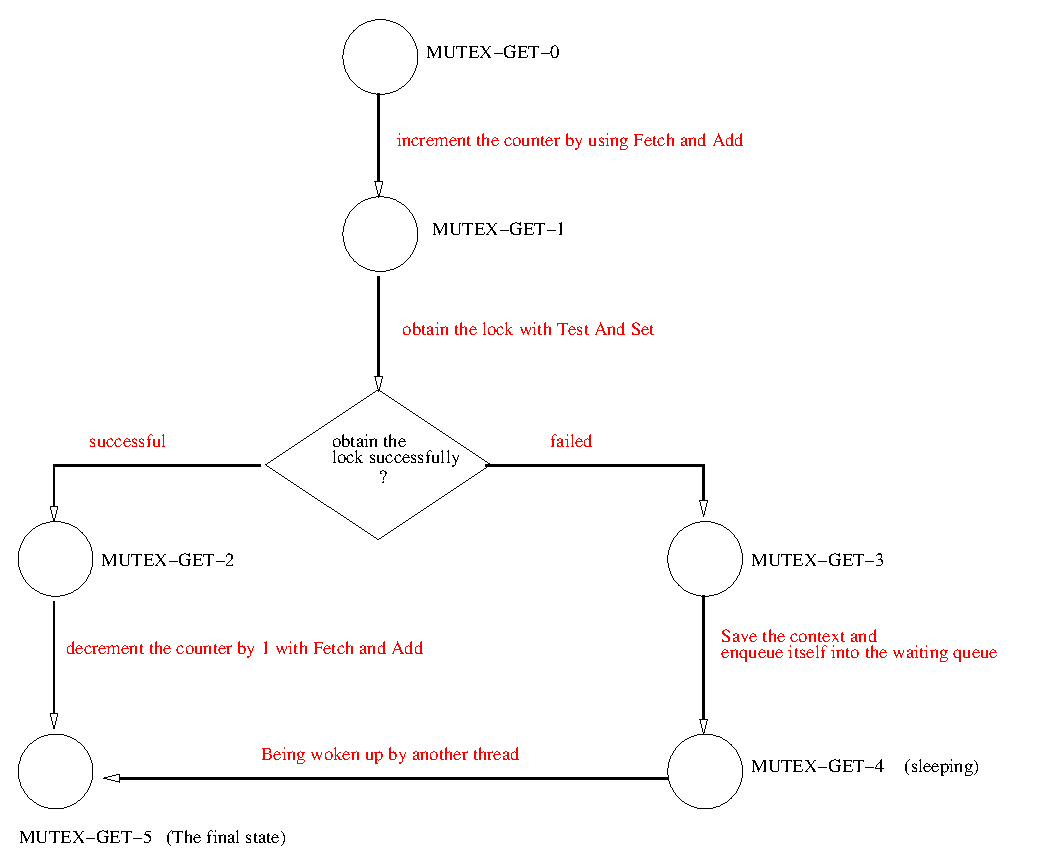
\includegraphics{mutex_get}


\end{figure}
%
\begin{figure}


\caption{State graph for the process of releasing a mutex}


\includegraphics{mutex_rel}


\end{figure}
\newpage{}


\section{Semaphores}

In this chapter, we will discuss implementations of semaphores for
SMASH. Although semaphores usually are considered to be a generalization
of mutexes, the implementations are different for efficiency reasons.
In fact, the need for a user level semaphore on SMASH is not as important
as that of the user-level mutex, because SMASH only creates as many
kernel threads as the number of CPUs we have. Hence for systems with
a small number of CPUs, for example a dual core or quad core machine,
if the semaphore is initialized to be more than 2 or 4 correspondingly,
then there will be no contention at all, but for a system with a large
number of CPUs, we believe that such implementations will still benefit
the entire system.


\subsection{APIs of user-level semaphores}


\subsubsection*{Semaphore initialization}

This function is used to initialize a given semaphore. It sets the
counter to the given number and creates a empty waiting queue. The
function is not thread safe.


\subsubsection*{Semaphore wait}

This function is used to perform the \emph{wait }function. It decrements
the counter by 1. If the result is negative, then the calling thread
has to wait in the waiting queue.


\subsubsection*{Semaphore signal}

This function is used to perform the \emph{signal }function. It increments
the counter by 1, then it checks whether there is any thread waiting
in the waiting queue. If so, it wakes one up. 


\subsection{Lock-based implementation for semaphores}

The semaphore can be considered to be a generalization of mutex. A
semaphore contains a counter. On initialization, this counter is set
to some initial number N, each wait operation decrements the counter
until it reaches zero, after which \emph{wait} operations will cause
the calling thread to be blocked in the waiting queue. A thread releases
the semaphore by calling the function \emph{signal}, which will increment
the counter by one if no other threads are waiting in the waiting
queue, or wake up a waiting thread. Here is the general data structure
of a semaphore.

%
\begin{algorithm}
\caption{General data structure of a semaphore}


struct sem\_t \{

~~int counter;

~~struct fifo waiting\_queue;

\}


\end{algorithm}


To implement semaphores, we have some similar issue to those of mutex,
the counter has to be updated atomically and the waiting queue has
to be thread-safe. On uniprocessor systems, we can still simply disable
interrupts to guarantee the atomicity of these operations, and on
SMP systems, we can use a spin lock to protect the critical sections.

%
\begin{algorithm}[H]
\caption{Lock-based semaphore implementation on SMP systems}


Wait(sem\_t s) \{

~~getSpinlock(s->spinlock);

~~if(s->counter <= 0)

~~~~save the current context;

~~~~enqueue(thread\_self, s->waiting\_queue);

~~~~releaseSpinlock(s->spinlock);

~~~~switch to the next runnable thread;

~~else

~~~~s->counter- -;

~~~~releaseSpinlock(s->spinlock);

\}\\


Signal(sem\_t s) \{

~~getSpinlock(s->spinlock);

~~if(s->counter > 0)

~~~~/{*} The resource is still available, no one is in the waiting
queue {*}/

~~~~s->counter++;

~~~~releaseSpinlock(s->spinlock);

~~~~return;

~~else 

~~~~/{*} The resource is not available, there may be some one
waiting in the waiting queue. {*}/

~~~~thread = dequeue(s->waiting\_queue);

~~~~if(thread != NULL)

~~~~~~wakeup(thread);

~~return;

\}
\end{algorithm}



\subsection{A Lock-free implementation}

To implement the lock-free version of semaphores, we have to consider
several issues. First, the counter has to be updated atomically, and
since the counter can take any integer value, we can not use \emph{Test\_and\_Set}
to update it, instead, we have to use other atomic instructions to
modify the counter. In addition, we still use a lock free FIFO queue
as the waiting queue.%
\begin{algorithm}
\caption{\emph{wait} function of the lock-free semaphore}


wait(sem\_t s) \{

~~~/{*} we may also use FetchAndAdd here, but I suspect that the
following code can improve the latency. {*}/

~~~do \{

~~~~~~counter = s->counter;

~~~\}while(!cas(\&s->counter,counter,counter-1));

~~~if(counter < 0)

~~~~~~/{*} The resouce is not available, wait in the waiting
queue {*}/

~~~~~~save the current contex;

~~~~~~enqueue(thread\_self, s->waiting\_queue);

~~~~~~switch to the next runnable thread;

~~~else

~~~~~~/{*} The resource is still available {*}/

~~~~~~return

\}


\end{algorithm}



\subsubsection{The \emph{lost-wake-up} problem}

In the implementation of the lock-free semaphore, we also have the
same \emph{lost-wake-up} problem as that in mutex implementation.
One of the threads holding the semaphore may fail to dequeue a waiting
thread from the waiting queue because at the time the thread checks
the waiting queue, it has not yet enqueued itself into the queue.
However, this time, the problem is harder to solve. Suppose that we
try to solve it with the same method that we used in the lock-free
mutex implementation. 

%
\begin{algorithm}[H]


\caption{Lost-wake-up problem}


L1~~~~signal(sem\_t s) \{

L2~~~~~~if(s->counter > 0)

L3~~~~~~~~FetchAndAdd(\&s->counter, 1);

L4~~~~~~else

L5~~~~~~~~do \{

L6~~~~~~~~~~~thread = dequeue(s->waiting\_queue);

L7~~~~~~~~~~~if(thread != NULL)

L8~~~~~~~~~~~~~wakeup(thread);

L9~~~~~~~~~~~~~return;

L10~~~~~~~while(thread == NULL);

L11~~~\}


\end{algorithm}


The problem is that in this case, we may have multiple dequeuers that
dequeue the waiting threads from the waiting queue. If one fails to
find any threads waiting in the queue, then there are two possibilities:
one is that the waiting thread has not yet inserted itself in the
queue, or maybe the waiting thread has been woken up by another thread
holding the semaphore. This may cause some threads loop forever trying
to dequeue a waiting thread while actually there is no one waiting. 

To solve this problem, we first allow the counter to take negative
integer values. If the counter takes a negative value, then its modulus
represents the number of threads waiting for the resource. When a
thread is trying to release the semaphore, it uses a loop in which
it first checks whether the counter is negative or not. If the counter
is non-negative, then it increments the counter by 1. Otherwise the
counter is negative, then there exists a thread waiting in the queue.
Hence the thread releasing the semaphore tries to dequeue a waiting
thread from the waiting queue. If it fails to get a waiting thread,
then it re-reads the counter and execute the loop again. The pseudo
code is shown in Algorithm \ref{alg:Incomplete-solution-to}.

%
\begin{algorithm}[!h]
\caption{\label{alg:Incomplete-solution-to}Incomplete solution to \emph{lost-wake-up}
problem}


L1~~~~signal(sem\_t s) \{

L2~~~~~~~do \{

L3~~~~~~~~~~~~if(s->counter < 0 )

L4~~~~~~~~~~~~~~~tmp\_thread = dequeue(s->waiting\_queue);

L5~~~~~~~~~~~~~~~if(tmp\_thread == NULL)

L6~~~~~~~~~~~~~~~~~~continue;

L7~~~~~~~~~~~~~~~else

L8~~~~~~~~~~~~~~~~~~FetchAndAdd(s->counter, 1);

L9~~~~~~~~~~~~~~~~~~wakeup(tmp\_thread);

L10~~~~~~~~~~~~~~~~~return;

L11~~~~~~~~~~~else

L12~~~~~~~~~~~~~~FetchAndAdd(s->counter,1);

L13~~~~~~~~~~~~~~return;

L14~~~~~~\}while(true);

L15~~~~\}


\end{algorithm}


However, this does not solve the problem completely, as there is another
race condition. Suppose a thread A holding the semaphore is trying
to release the resource, and it just finishes L3 with the counter
greater than zero. The next instruction to be run should be L12, but
before the counter is incremented, suppose the resource is used up
and some threads have enqueued themselves into the waiting queue.
Then at least one of the waiting thread will not be woken up, i.e.
we again have the \emph{lost-wake-up} problem. To solve this problem,
we have to guarantee that the process of testing the counter and updating
it if it is not negative should be atomic. Hence, we use an outer
do-while loop surrounding the do-while loop in the above pseudo code
and use \emph{Compare\_And\_Swap} to update the counter. %
\begin{algorithm}
\caption{Proper implementation for \emph{signal} on the lock-free semaphore}


L1~~~~signal(sem\_t s) \{

L2~~~~~~~do\{

L3~~~~~~~~~~~~~old = s->counter

L4~~~~~~~~~~~~~do \{

L5~~~~~~~~~~~~~~~~~~if( s->counter< 0 )

L6~~~~~~~~~~~~~~~~~~~~~tmp\_thread = dequeue(s->waiting\_queue);

L7~~~~~~~~~~~~~~~~~~~~~if(tmp\_thread == NULL)

L8~~~~~~~~~~~~~~~~~~~~~~~~continue;

L9~~~~~~~~~~~~~~~~~~~~~else

L10~~~~~~~~~~~~~~~~~~~~~~~FetchAndAdd(\&s->counter,
1);

L11~~~~~~~~~~~~~~~~~~~~~~~wakeup(tmp\_thread);

L12~~~~~~~~~~~~~~~~~~~~~~~return;

L13~~~~~~~~~~~~~~~~~else

L14~~~~~~~~~~~~~~~~~~~~break;

L15~~~~~~~~~~~~\}while(true);

L16~~~~~~\}while(!CAS(\&s->counter,old,old+1))

L17~~~~\}
\end{algorithm}



\subsubsection{Correctness analysis}

Lock-free semaphores are more complicated than lock-free mutexes.
We divide the process of waiting on a semaphore into five states:
SEM-WAIT-0, SEM-WAIT-1,SEM-WAIT-2, SEM-WAIT-3, SEM-WAIT-4, and divide
the process of signaling a semaphore into six states: SEM-SIG-0, SEM-SIG-1,
SEM-SIG-2, SEM-SIG-3, SEM-SIG-4, SEM-SIG-5. To check the safety property,
we first identify the bad combinations of states. Suppose the counter
of the semaphore was initialized to be N. The first bad combination
is that there are more than N threads in SEM-WAIT-4, i.e. there are
more than N threads accessing the resource protected by the semaphore.
The second bad combination is the case in which the counter of the
semaphore is greater than or equal to zero, but there still exist
threads waiting in the waiting queue, i.e. we have the \emph{lost-wake-up}
problem. The third one is that a thread is in the state SEM-REL-3
but the counter is non-negative. In this case the thread will loop
forever trying to wake someone up but there is actually no one in
the waiting queue.

The first case is not possible. Because if the counter is less than
zero, then a thread A trying to obtain the semaphore has to wait in
the waiting queue, even another thread B holding the semaphore released
the resource just after the time thread A checked the counter. In
this case, A has to insert itself into the waiting queue and wait
for other thread to wake it up. The second case will not happen because
for each thread waits in the waiting queue, they have already decremented
the counter so that it is negative, and the counter will not be incremented
unless one of the waiting threads is woken up successfully. Even in
the case that the counter becomes negative when a thread holding the
resource is in the state SEM-REL-1, it will not be able to update
the counter successfully since the counter is updated with \emph{Compare\_And\_Swap},
and consequently it will go back to SEM-REL-0. The last situation
is also impossible because once a thread holding the resource fails
to dequeue a waiting thread from the waiting queue, it rechecks the
counter. If the counter is not negative any more, then the execution
goes back to SEM-REL-0.%
\begin{figure}
\caption{State graph for the \emph{wait} function on the lock-free semaphore}


\includegraphics[scale=0.8]{sem_wait}
\end{figure}
%
\begin{figure}
\caption{State graph of the \emph{signal} function on the lock-free semaphore}


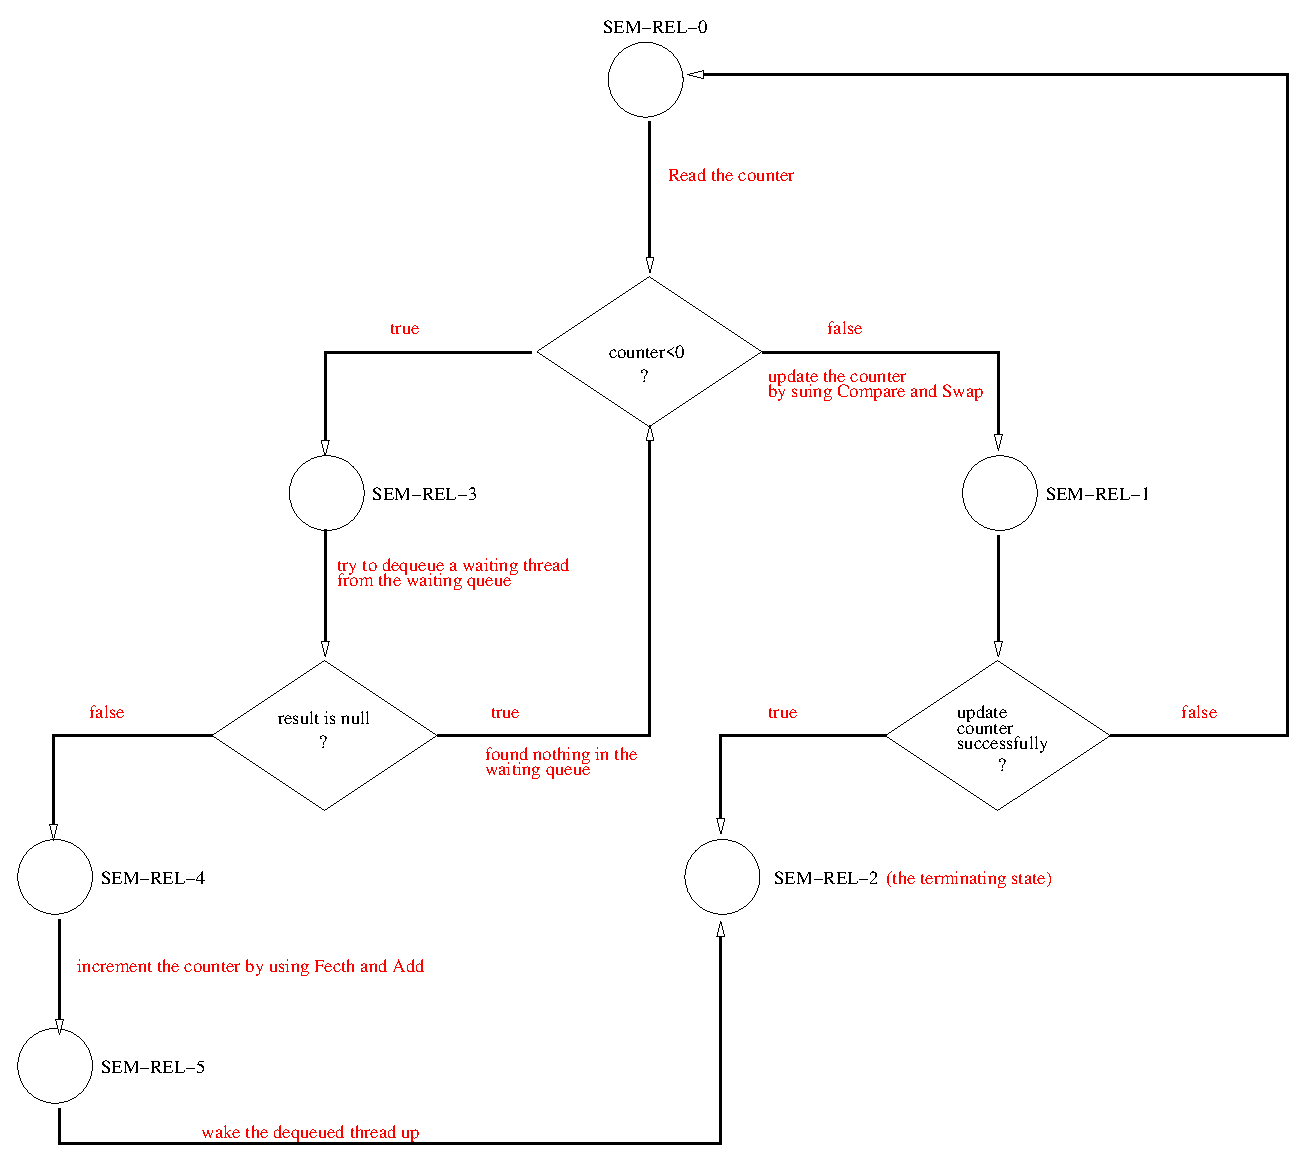
\includegraphics[scale=0.7]{sem_sig}
\end{figure}
\newpage{}


\section{Message queues}

In this chapter, we will discuss implementations of message queues.
The message queues we implemented are unbounded, multiple sender,
single dequeuer queues. Unboundedness means that these queues are
potentially capable of storing infinitely many messages, since the
only limit is the memory space. Also there can be more than one sender
that send messages to the queue, but there is only one receiver. If
the receiver tries to retrieve a message from a empty queue, it blocks
until a sender wakes it up. 


\subsection{APIs of message queues}


\subsubsection*{Message queue initialization}

This function initializes a message queue. It creates an empty FIFO
queue to store messages and sets the other field in the message queue
to the initial values.


\subsubsection*{Send message}

Given the memory address of a message, this function creates a new
node to store the message and enqueues the node to the given message
queue, if the receiver is waiting for the message, it will wake the
waiting thread up.


\subsubsection*{Fetch message}

The receiver of a message queue calls this function to dequeue a message
from the message queue, if the queue is empty, then the receiver will
block until a message is available. This function returns the address
where the message is stored in the memory, and it automatically destroys
the dequeued node structure by using the function \emph{free}.


\subsection{Lock-based implementation}

The lock-based approach is quite simple, as we just use a spin lock
to protect the queue. Note that it is not enough to just protect the
FIFO queue which is used to store the message, because it is possible
that we encounter a situation where a sender just inserts a message
into an empty queue and find no one is waiting, but the real case
is that the receiving thread is in the process of saving its context
and making itself wait on the message queue because the queue was
empty at the time it was checked. In this case, we again suffer from
the \emph{lost-wake-up} problem. Hence, a spin lock is used to protect
the entire function calls of \emph{Send\_message} and \emph{Fetch\_message}.
In this way, it is guaranteed that when the receiver is fetching the
message and the message is empty, a sender will not be able to send
the message until the receiver is waiting for the message. 

Since the entire processes of sending and receiving messages are protected
by a spin lock, we can use a simple FIFO queue as the queue storing
the messages. The FIFO queue is implemented as a single linked-list
with a dummy head node. Each node contain a \emph{data} pointer pointing
to the memory location where the actual message is stored and a \emph{next
}pointer which points to the next node in the FIFO queue. %
\begin{algorithm}


\caption{Structure for nodes of the FIFO queue}


struct fifo\_node \{

~~~void {*} data\_pointer;

~~~struct fifo\_node {*} next;

\}


\end{algorithm}
The queue itself has two pointers: the \emph{head} pointer pointing
to the head node of the queue, and the \emph{tail} pointer pointing
to the tail node. Initially, both head and tail pointers point to
the dummy. The enqueue operation appends a new node to the tail of
the list and the dequeue operation removes the current dummy head
from the queue and makes the next node be the new dummy head.

When a sender sends a message, it uses \emph{malloc }to create a new
node in the heap and enqueue the new node to the message queue. Then
the receiver will dequeue the message and use \emph{free }to free
the space allocated to the old dummy head. Since nodes only store
pointers to actual messages, the length of messages can be arbitrary.
It is up to the application developer who uses the message queue to
decide the detailed structures of messages.

%
\begin{algorithm}[H]
\caption{Lock-based message queue}


struct message\_queue \{

~~int spinlock;

~~struct fifo queue;

~~cthread waiting\_thread;

\}\\


Send\_message(message, message\_queue q) \{

~~getSpinlock(q->spinlock);

~~enqueue(message,q->queue);

~~if(q->waiting\_thread != NULL)

~~~~/{*} no thread is blocking {*}/

~~~~tmp\_thread = q->waiting\_thread;

~~~~q->waiting\_thread = NULL;

~~~~wakeup(tmp\_thread);

~~releaseSpinlock(q->spinlock);

~~return;

\}\\


Fetch\_message(message\_queue q) \{

~~getSpinlock(q->spinlock);

~~message = dequeue(q->queue);

~~if(message == NULL)

~~~~/{*} The message queue is empty, we wait. {*}/

~~~~save the current context;

~~~~q->waiting\_thread = thread\_self;

~~~~releaseSpinlock(q->spinlock);

~~~~switch to the next runnable thread;

~~releaseSpinlock(q->spinlock);

~~return message;

\}
\end{algorithm}



\subsection{Lock-free implementation}

To implement the lock-free message queue, there are two issues to
solve. The first one is that the FIFO queue has to be thread safe,
the second one is the \emph{lost-wake-up} problem. The former issue
can be solved by using a lock-free FIFO queue. In order to solve the
lost-wake-up problem, an extra field, called \emph{waiting\_mark,
}is added to the message queue structure. When a receiver fetches
a message from the queue, it first sets the mark to WAITING, then
it performs the dequeue operation. If the result is NULL, then it
blocks. Otherwise, the result is not NULL, then the function resets
\emph{waiting\_mark }to NOWAITING and returns the result. When a sender
sends a message to a message queue, it first enqueues the node containing
the message to the queue. Then it uses a \emph{do-while }loop, which
ends if the value of \emph{waiting\_mark} is not WAITING, to try to
wake up the receiver(if any). In the loop, the thread first swaps
NULL into the field \emph{waiting\_thread} and if its old value is
not NULL, then it wakes up the receiver and sets the field \emph{waiting\_mark
}to NOWAITING. 

%
\begin{algorithm}


\caption{The data structure of the lock-free message queue }


struct message\_queue \{

~~struct lockfree\_fifo {*} queue;

~~cthread {*} waiting\_thread;

~~int waiting\_mark;

\}


\end{algorithm}
%
\begin{algorithm}
\caption{\emph{Fetch\_message} function of the lock-free message queue}




Fetch\_message(struct message\_queue {*} q) \{

~~while(true) \{

~~~~queue->waiting\_mark = WAITING; /{*} This means that the receiver
is fetching messages {*}/

~~~~result = dequeue(q->queue);

~~~~if(result == NULL)

~~~~~~/{*} The queue is empty. {*}/

~~~~~~save the current context;

~~~~~~q->waiting\_thread = thread\_self;

~~~~~~switch to the next runnable thread;

~~~~~~continue on wakeup

~~~~else

~~~~~~queue->waiting\_mark = NOWAITING; /{*} denote that no
one is waiting {*}/

~~~~~~reture result;

\}
\end{algorithm}
%
\begin{algorithm}
\caption{\emph{Send\_message} of the lock-free message queue}


Send\_message(message, struct message\_queue q) \{

~~enqueue(message, q->queue);

~~do \{

~~~~~~~~thread = swap(\&queue->waiting\_thread,NULL);

~~~~~~~~if(thread != NULL)

~~~~~~~~~~~/{*} Do NOT exchange the order of the following
instructions,

~~~~~~~~~~~~~~because it will lead to a potential race
condition {*}/

~~~~~~~~~~~queue->waiting\_mark = NOWAITING;

~~~~~~~~~~~wakeup(thread);

~~while(queue->waiting\_mark == WAITING);

\}


\end{algorithm}



\subsubsection{Correctness}

We divide the the process of sending a message into 5 states: QUEUE-SEND-1,
QUEUE-SEND-2, QUEUE-SEND-3, QUEUE-SEND-4, QUEUE-SEND-5, and the process
of fetching a message into 6 states: QUEUE-FETCH-1, QUEUE-FETCH-2,
QUEUE-FETCH-3, QUEUE-FETCH-4, QUEUE-FETCH-5, QUEUE-FETCH-6. And we
produce the state diagrams for them.%
\begin{figure}
\caption{The state diagram for sending messages}


~~~~~~~~~~~~~~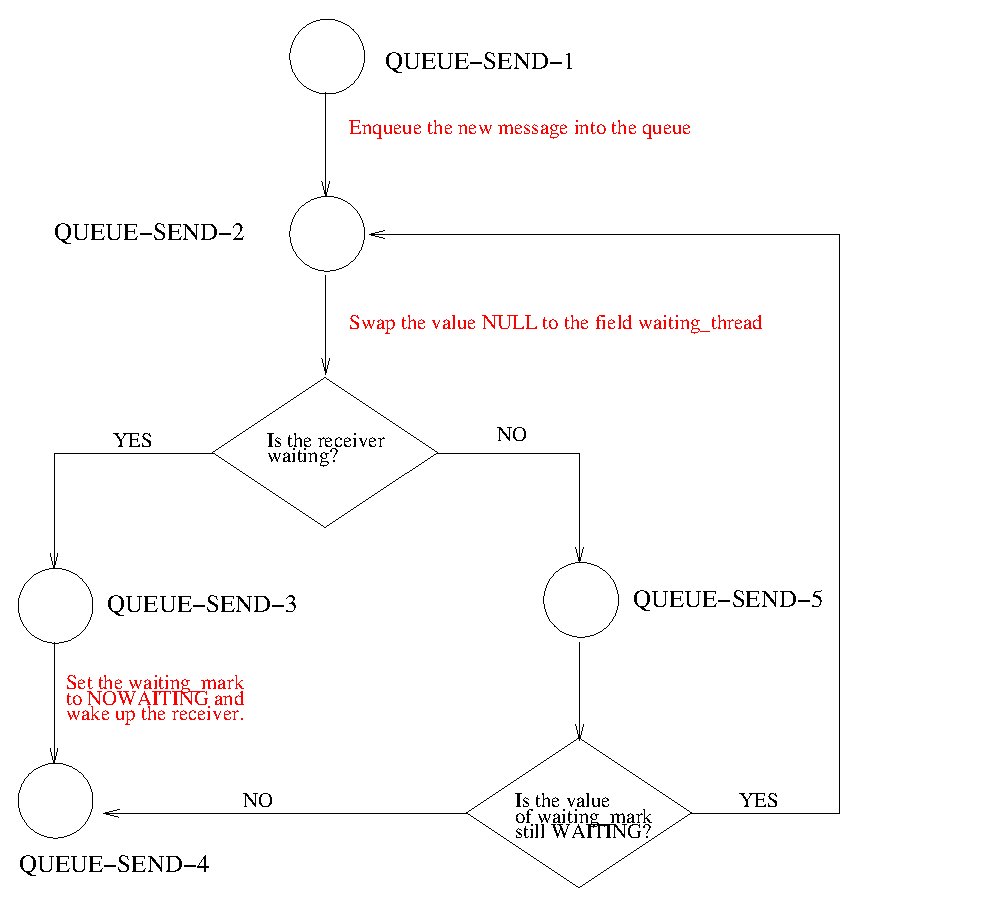
\includegraphics[scale=0.8]{queue_send}


\end{figure}
%
\begin{figure}
\caption{The state diagram for fetching messages}


~~~~~~~~~~~~~~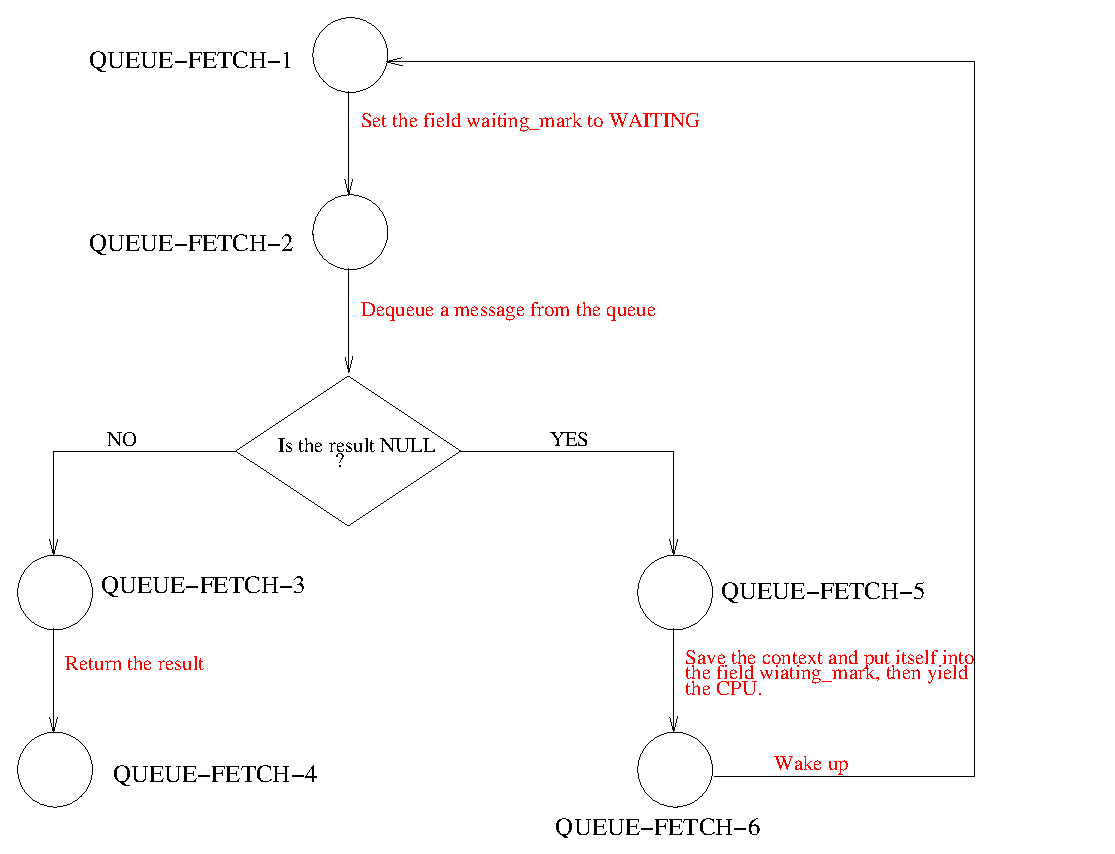
\includegraphics[scale=0.8]{queue_fetch}


\end{figure}


In this case, the only problem is the \emph{lost-wake-up }problem.
And it will not happen because before the receiver of a message queue
tries to fetch a message from the queue, it sets the field \emph{waiting\_mark
}to the value WAITING. And as long as the value of \emph{waiting\_mark}
is still WAITING, senders will keep looping to check the field \emph{waiting\_thread}.
If its value is not NULL, which means the receiver has blocked or
is in the process of blocking on the message queue, then one of the
sender will reset the \emph{waiting\_mark }field to NOWAITING and
then wake the receiver up. If the receiver gets a message successfully
in the first place, then it will reset the \emph{waiting\_mark }to
NOWAITING.

\newpage{}


\section{Channels}

In this chapter, we implemented the CSP communication channels designed
by Vella\cite{15} for KRoC. KRoC is an implementation of the OCCAM
2 programming language\cite{28}. OCCAM is a concurrent programming
language which is built on the communicating sequential process algebra.
Channels here have the same semantics as those in the OCCAM 2 programming
language. 


\subsection{Semantics of channels}

Channels are used for unbuffered synchronized communications between
threads. A channel has two ends, the input end and the output end.
At any time, only one thread can read input from a channel and only
one thread can output to the channel. Also the communication is synchronized,
which means the communication will not happen until the two ends are
both ready, and the message is copied directly from the outputting
thread to the inputting thread. That means there is no intermediate
buffer between them. If one of the communication ends is not ready
to take action, then the other end will block to wait for it. %
\begin{figure}


\caption{Example of channel communication}


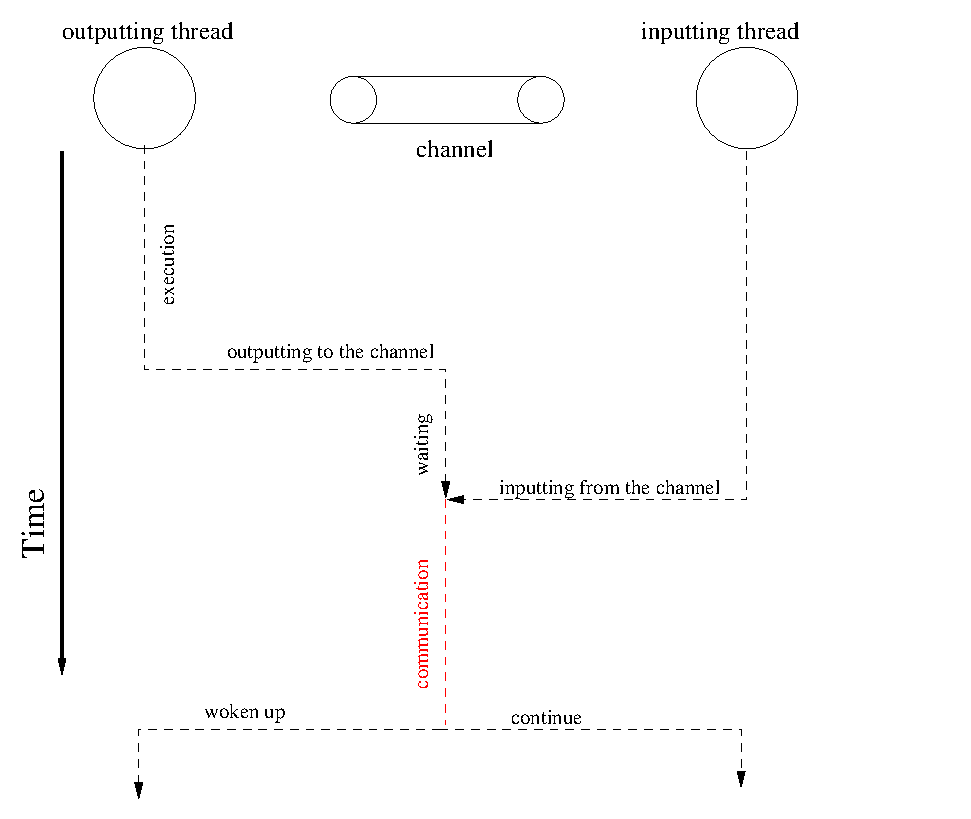
\includegraphics{chan_out_wait}


\end{figure}
 This enforces determinism, since we know when the communication will
happen and the source and the destination of the communication. 

However, in some cases, we may need the communication to be non-deterministic,
for example, a web server waiting for client requests. In this case,
the server will not be able to know which client will send the request
first. OCCAM provides \emph{alternatives }to cater for this situation.
\emph{Alternatives} allow an input thread wait on a set of channels
for communication. When one of the channels is ready, the communication
will happen on that channel. If none of them is ready at the time
the inputting thread is trying to receive messages, then the inputting
thread sleeps until one of the channels is ready. On the other hand,
if more than one channel is ready at the same time, the inputting
thread will pick one of them. In theory, the choice should be totally
nondeterministic, but it is hard to implement efficiently, so in practice,
the choice is made in a deterministic manner. %
\begin{figure}


\caption{Alternative of channels}


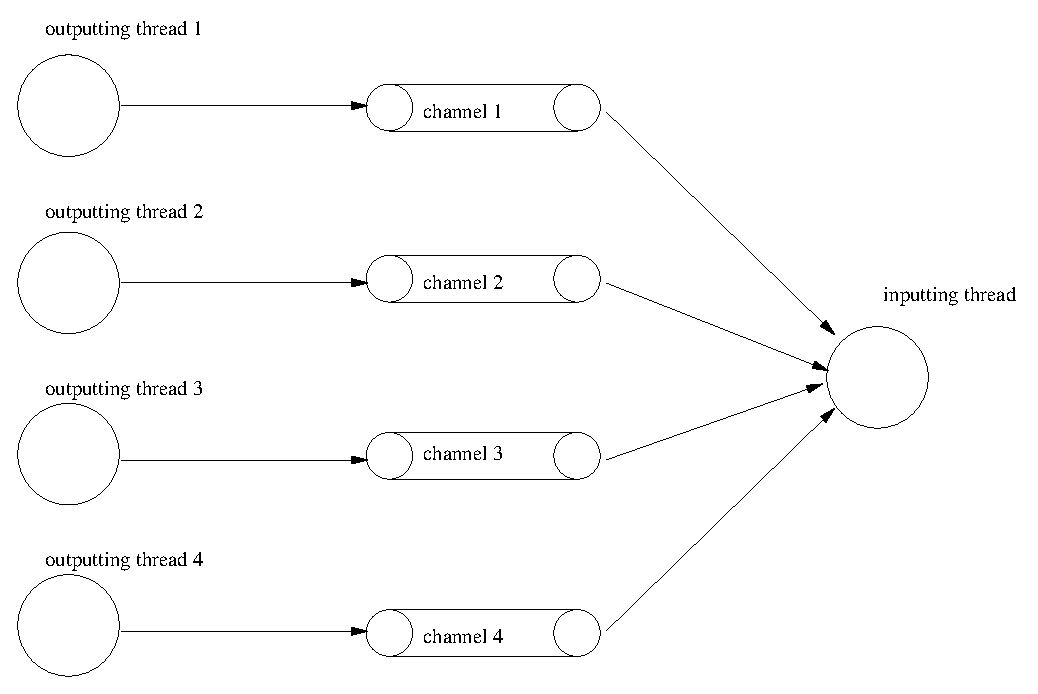
\includegraphics[scale=0.9]{alt}


\end{figure}



\subsection{APIs for channels}


\subsection*{Channel input with alternative}

This function is used when a thread tries to take input from an array
of channels, and it follows the same semantics as described in the
above section. This function can be used for simple channel communication,
but it is different from the channel implementation provided by SMASH,
since \emph{alternative }is always enabled.


\subsection*{Channel output with alternative}

This function is used when a thread tries to output on a channel.
\emph{Alternative support }is always enabled even in the case of simple
channel communications.


\subsection{Simple Channel communication}

SMASH provides lock-based and wait-free implementations of channels
for simple channel communications. These channels do not support alternatives.
They are tightly integrated with SMASH, since in the thread descriptor
structure of SMASH, there is a pointer used to pointing to the memory
address of the message and the length of a message is also recorded
in this structure. Messages are copied directly from one thread to
the other. %
\begin{algorithm}


\caption{Data structure for wait-free channels without alternative support}


struct channel \{

~~~cthread {*} communicator

\}
\end{algorithm}
%
\begin{algorithm}
\caption{Wait-free channel input}


channel\_in(channel chan, int n) \{

~~~save the current context

~~~if(CAS(chan->communicator, NULL, self))

~~~~~~schedule the next runnable thread

~~~~~~return on wakeup

~~~else

~~~~~~copy n bytes from chan->communicator->message

~~~~~~chan->communicator = NULL

~~~~~~wakeup(chan->communicator)

~~~~~~return

\}
\end{algorithm}
%
\begin{algorithm}
\caption{Wait-free channel output}


channel\_out(channel chan, int n) \{

~~save the current context

~~if(CAS(chan->communicator,NULL self))

~~~~// The inputting thread has not reached the communication
point yet, we sleep.

~~~~schedule the next runnable thread

~~~~return on wakeup

~~else

~~~~copy n bytes TO chan->communicator->message

~~~~chan->communicator = NULL

~~~~wakeup(chan->communicator)

~~~~return

\}


\end{algorithm}



\subsection{Lock-based Channels with alternative support}

In this section, we implemented channel communication with alternative
support by using spin locks. Our design is quite simple, the set of
channels participating the communication are grouped together into
a data structure called \emph{channel set, }when a thread tries to
input from the set of channels, it uses a spin lock to lock the entire
set, then it checks whether there is a channel in the set ready for
communication, i.e. the outputting thread is waiting on that channel,
if a channel is ready, then the inputting thread copies the message
from the channel and wakes up the outputting thread. If none of the
channels is ready, then it blocks on all these channels.

When an outputting thread tries to output on a channel, it also locks
the entire set of channels, then it check if the inputting thread
is ready for communication, if the inputting thread is ready, then
it copies the message to that thread and wakes it up, after which,
the outputting thread loops over all these channels, if it finds that
the inputting thread is also waiting on other channels, it will disable
these channels by setting the \emph{channel communicator} field to
NULL. Then it wakes up the inputting thread and releases the spin
lock. If the channel is not ready for communication, it releases the
spin lock and blocks itself on the channel.%
\begin{algorithm}[H]


\caption{Data structure for \emph{channel set}}


struct channel\_set \{

~~channel {*}{*} chan\_array;

~~int chan\_num;

~~int spinlock;

\}


\end{algorithm}
%
\begin{algorithm}[H]
\caption{Lock-based channel input with alternative support}


channel\_in(channel\_set {*} chan\_set, void {*} message, int length)
\{

~~getSpinlock(chan\_set->spinlock);

~~save the current context;

~~for(count = 0; count < chan\_set->chan\_num; count++)

~~~~if(chan\_set->chan\_array{[}count]->communicator != NULL)

~~~~~~copy message from the channel;

~~~~~~chan\_set->chan\_array{[}count]->communicator = NULL;

~~~~~~wake up the communicator;

~~~~~~releaseSpinlock(chan\_set->spinlock);

~~~~~~return;

~~for(count = 0; count < chan\_set->chan\_num; count++)

~~~~chan\_set->chan\_array{[}count]->communicator = thread\_self;

~~releaseSpinlock(chan\_set->spinlock);

~~schedule the next runnable thread;

\}


\end{algorithm}
%
\begin{algorithm}[H]


\caption{Lock-based channel output with alternative support}


channel\_out(channel\_set {*} chan\_set, int index, void {*} message,
int length) \{

~~getSpinlock(chan\_set->spinlock);

~~save the current context;

~~input\_thread = chan\_set->chan\_array{[}index]->communicator; 

~~if(input\_thread != NULL)

~~~~copy message to the channel;

~~~~for(count = 0; count < chan\_set->chan\_num; count++)

~~~~~~if(chan\_set->chan\_array{[}count]->communicator == input\_thread)

~~~~~~~~chan\_set\_>chan\_array{[}count]->communicator = NULL;

~~~~wake up input\_thread;

~~~~releaseSpinlock(chan\_set->spinlock);

~~~~return;

~~else

~~~~chan\_set->chan\_array{[}index]->communicator = thread\_self;

~~releaseSpinlock(chan\_set->spinlock);

~~schedule the next runnable thread;

\}


\end{algorithm}



\subsection{Wait-free Channels with alternative support}

Vella designed a wait-free channel for KRoC in his PhD thesis\cite{15},
and in this project, we ported it to SMASH. The algorithm is array-based,
which means that the number of channels that participate in the alternative
is fixed and is known before the communication starts. In the design,
the only atomic instruction used is \emph{Swap.} When a thread outputs
to a channel, it first saves its current context, then uses swap instruction
to get the current value of the channel communicator and insert itself
to the \emph{communicator} field. Then it checks if the value it got
is NULL or not. If the value is NULL, then it means that at the time
of the execution of the \emph{swap} instruction, the inputting thread
had not reached the communication point yet, so the outputting thread
goes to sleep. If the channel communicator was not NULL, i.e. the
inputting thread had insert itself to the \emph{communicator} field
of the channel, the outputting thread then uses \emph{swap} again
to read the old value of the field \emph{pointer }in the inputting
thread structure and sets its new value to READY atomically, then
it checks the old value. If the old value was ENABLING or READY, then
it goes to sleep, while if the old value was WAITING, which means
the inputting thread is sleeping or is in the process of sleeping,
so it should be woken up again. If the old value is none of the above
values, it means that the alternative is disabled, i.e. the communication
is just a simple channel communication, then the mechanism of simple
channel communications is applied. 

When a thread inputs from a group of channels, the entire process
is divided into three phases: 

\begin{enumerate}
\item The enabling phase,
\item The alternative waiting phase, 
\item The disabling phase.
\end{enumerate}
In the enabling phase, the inputting thread first sets the \emph{pointer
}field in its thread structure to ENABLING, then it loops over the
set of channels. For each channel, it uses \emph{swap }to retreive
the old value of the channel communicator and insert itself to the
\emph{communicator} field, then it checks whether the old value is
NULL or not. If the old value was not NULL, then it sets its \emph{pointer}
field to READY and resets the channel communicator to its old value.
This process is done for every channel participating in the communication.
One thing to note is that in this phase, the inputting thread does
not need to save its context.

The second phase is the alternative phase, in this phase, the inputting
thread first sets its \emph{temp }field in the thread structure to
NULL and saves its current context, then it uses \emph{swap }to get
the old value of the \emph{pointer} field and sets its new value to
WAITING. After that, it checks the old value, and if the value was
ENABLING, we then go to the disabling phase. If the value was READY,
then it swaps\emph{ }the value READY back to the \emph{pointer }field
and gets the previous value atomically. If the newly retrieved value
is also READY, that means the \emph{pointer} field has been changed
by the outputting thread during L5, so we have to go to sleep since
the outputting thread will wake us up anyway. If the value retrieved
at L6 is not READY, then we should go to the third phase. 

The last phase is the disabling phase. During this phase, the inputting
thread chooses one of the ready channels to complete the communication
and disables all other channels. It is guaranteed that if a inputting
thread enters this phase, then there exists a channel that is ready
for the communication. In this phase, the inputting thread loops against
the channel array to swap the value NULL to the channel communicator
field one by one and checks the swapped value. If the value is the
memory address of the inputting thread's thread structure, then it
does nothing. If the swapped value is some other value, i.e. it is
the address of an outputting thread, and the \emph{temp }field of
the inputting thread is still NULL, then we set the \emph{temp} field
to that value to denote that the corresponding channel is chosen for
communication. If the value of \emph{temp }is not NULL, which means
a channel is already chosen, then we put the outputting thread back
into the channel communicator field.%
\begin{algorithm}[H]
\caption{Enabling phase of channel input}


channel\_enable(channel chan\_array, int array\_size) \{

L1~~~~/{*}Enabling alternative support.{*}/

L2~~~~thread\_self->pointer = ENABLING

~~~~~~/{*} Loop against channel array to check whether any channel
is ready. 

~~~~~~~~~i.e. some outputting threads have already been waiting
on the 

~~~~~~~~~corresponding channels {*}/

L3~~~~for(count = 0; count < array\_size; count ++)

L4~~~~~~~~temp\_thread = swap(chan\_array{[}count]->communicator, 

~~~~~~~~~~~~~~~~~~~~~~~~~~~~~~~thread\_self)

L5~~~~~~~~if(temp\_thread != NULL)

L6~~~~~~~~~~~/{*} This channel is ready {*}/

L7~~~~~~~~~~~thread\_self->pointer = READY

L8~~~~~~~~~~~chan\_array{[}count]->communicator = temp\_thread

\}
\end{algorithm}
%
\begin{algorithm}[H]
\caption{Alternative waiting phase for channel input}


alt\_wait(channel chan\_array, int array\_size) \{

L1~~~/{*} Start alternative wait phase {*}/

L2~~~thread\_self->temp = NULL

L3~~~save the current context

~~~~/{*} put the value WAITING to thread\_self->pointer 

~~~~~~~and retrieve its previous value atomically by using
swap {*}/

L4~~~temp = swap(thread\_self->pointer, WAITING)

L5~~~if(temp == READY)

~~~~~~~~/{*} one of the channels is ready, change the value
back to READY {*}/

L6~~~~~~temp = swap(thread\_self->pointer, READY)

L7~~~~~~if(temp == READY)

~~~~~~~~~~/{*} some outputting thread just changed the value 

~~~~~~~~~~~~~and try to wake us up while we are not sleeping, 

~~~~~~~~~~~~~so release the CPU {*}/

L8~~~~~~~~schedule the next runnable thread

L9~~~~~~~~return on wake up

L10~~else if (temp == ENABLING)

~~~~~~~~~~/{*} No channel is ready yet {*}/

L11~~~~~~~schedule the next runnable thread

L12~~~~~~~return on wake up

\}
\end{algorithm}
%
\begin{algorithm}[H]
\caption{Disabling phase for channel input}


channel\_disable(channel chan\_array, int array\_size) \{

/{*} Disabling all channels and choose one channel from the ready
ones to finish the communication {*}/

L1~~~for(count = 0; count < array\_size; count++)

L2~~~~~~~temp\_thread = swap(chan\_array{[}count]->communicator,
NULL)

L3~~~~~~~if(temp\_thread == thread\_self)

L4~~~~~~~~~~continue

L5~~~~~~~else

L6~~~~~~~~~~if(thread\_self->temp == NULL)

~~~~~~~~~~~~~/{*} This channel is ready and no channel
has been selected, 

~~~~~~~~~~~~~~~~we can choose this one {*}/

L7~~~~~~~~~~~~~thread\_self->temp = temp\_thread

L8~~~~~~~~~~else

L9~~~~~~~~~~~~~chan\_array{[}count]->communicator = temp\_thread

\}
\end{algorithm}
%
\begin{algorithm}[H]
\caption{ channel input of the wait-free channel}


channel\_in\_alt(channel chan\_array, int array\_size, void {*} message,
int length)

\{

~~channel\_enable(chan\_array,array\_size)

~~alt\_wait(chan\_array,array\_size)

~~channel\_disable(chan\_array,array\_size)

~~copy message from thread\_self->temp

~~wake up thread\_self->temp

\}
\end{algorithm}
%
\begin{algorithm}[H]
\caption{Channel out for wait-free channels}


channel\_out(channel chan, void {*} message, int length) \{

~~save the current context

~~temp\_thread = swap(chan->communicator, thread\_self)

~~if(temp\_thread == NULL)

~~~~~schedule the next runnable thread

~~~~~return on wake up

~~else

~~~~temp\_pointer = swap(temp\_thread->pointer,READY)

~~~~switch(temp\_pointer) \{

~~~~case ENABLING:

~~~~case READY:

~~~~~~~~~schedule the next runnable thread

~~~~~~~~~return on wake up

~~~~case WAITING:

~~~~~~~~~wake up temp\_thread

~~~~~~~~~schedule the next runnable thread

~~~~~~~~~return on wake up

~~~~default:

~~~~~~~~~copy message to temp\_thread->pointer

~~~~~~~~~return

\}
\end{algorithm}



\subsubsection{Correctness}

The correctness of this wait-free channel has been proved in \cite{11},
so we are not going to give an analysis. Instead, we just give state
diagrams for the enabling phase and the alternative waiting phase.
The disabling phase is very simple so we do not give a diagram for
it.%
\begin{figure}[H]
\caption{Enabling phase of channel input}


~~~~~~~~~\includegraphics[scale=0.8]{chan_in_enabling}


\end{figure}
%
\begin{figure}[H]
\caption{Alternative waiting phase of channel input}


\includegraphics[scale=0.8]{chan_in_alt}


\end{figure}



\section{Conclusion}

In this chapter, we discussed the designs and implementations for
user-level mutexes, semaphores, message queues and the CSP channels.
As we can see, the lock-based designs are all relatively simple and
the correctness is easy to check. In contrast, The lock-free implementations
are more complicated, and to check the correctness, simple analysis
is not enough. Instead, rigorous mathematical proofs have to be done
to guarantee the correctness. In the next chapter, we are going to
present some benchmarks about these constructs and give some analyze
the performance.


\chapter{Performance}

In this chapter, we will give a performance analysis for all inter-thread
communication constructs introduced in this dissertation. For each
kind of construct, both the lock-based and lock-free implementation
are used. The machine we used is a laptop equipped with a Intel Core2
Duo 1.83Ghz CPU with 4Mb L2 cache, 2Gb memory. The operating system
is Debian GNU/Linux unstable with Linux kernel version 2.6.24. The
compiler is GCC 4.3. When measuring these benchmarks, we try to run
as few programs as possible, the largest program running being the
X-window system.


\section{Benchmarks for mutex}

Originally, SMASH did not implement the user-level mutex, so when
a mutex was needed, one had to user either pthread's mutex or a spin
lock directly. Either way, if the mutex or spin lock is under contention,
not only does the user-level thread block, but so does the underlying
kernel, and consequently, no other user-level threads can run on that
kernel thread. In the worst case, all kernel threads except the one
on which the user-level thread holding the mutex will be blocked.
This will slow down the entire system. 

We created six identical independent tasks, each of which contains
nothing but a critical section protected by a mutex. In the critical
section, a thread loops to increment a counter which is not shared.
For each critical section, we create ten user-level threads working
on it. The program loops for a number which is defined by GRANULARITY.
We used a pthread mutex and our lock-free mutex to analyze the performance.
It is desirable that the choice of different implementations of user-level
mutexes will not make a significant difference since we are measuring
the performance of the entire system, not that of mutexes. %
\begin{algorithm}
\caption{The benchmark of the system using lockfree user-level mutex}


\#define TASK\_NUM 6 

\#define THREAD\_PER\_TASK 10 

\#define STEP 500000 

int GRANULARITY = STEP; 

cmutex\_t m{[}TASK\_NUM]; 

long task{[}TASK\_NUM]; 

void test(cthread {*} ct,int task\_num) \{ 

~~~int count,n=0; 

~~~GetMutex(\&m{[}task\_num]); 

~~~for(count=0;count < GRANULARITY;count++) 

~~~~~~n++; 

~~~ReleaseMutex(\&m{[}task\_num]); 

~~~cthread\_stop(); 

\}

void cthread\_main() \{ 

~~~int count,i=0,thread\_num = THREAD\_PER\_TASK {*} TASK\_NUM; 

~~~int thread\_count = 0; 

~~~struct timeval t1,t2; 

~~~cthread {*} c{[}TASK\_NUM]{[}THREAD\_PER\_TASK]; 

~~~for(count=0;count<TASK\_NUM;count++) 

~~~~~cmutex\_init(\&m{[}count]); 

~~~while(i<10) \{ 

~~~~~gettimeofday(\&t1,NULL); 

~~~~~for(count=0;count<TASK\_NUM;count++) 

~~~~~~~for(thread\_count=0;thread\_count<THREAD\_PER\_TASK;

~~~~~~~~~~~thread\_count++) 

~~~~~~~~~c{[}count]{[}thread\_count] = cthread\_init(test,4096,1,count); 

~~~~~for(count=0;count<TASK\_NUM;count++) 

~~~~~~~for(thread\_count=0;thread\_count<THREAD\_PER\_TASK;

~~~~~~~~~~~thread\_count++)

~~~~~~~~~cthread\_run(c{[}count]{[}thread\_count]);

~~~~~for(count=0;count<TASK\_NUM;count++)

~~~~~~~for(thread\_count=0;thread\_count<THREAD\_PER\_TASK;

~~~~~~~~~~~thread\_count++) 

~~~~~~~~~cthread\_join(c{[}count]{[}thread\_count]); 

~~~~~gettimeofday(\&t2,NULL); 

~~~~~printf(\char`\"{}Main Thread:time cost:\%f, Granularity:\%d\textbackslash{}n\char`\"{},

~~~~~~~~~~~~~calculate(t1,t2),GRANULARITY); 

~~~~~i++; 

~~~~~GRANULARITY = GRANULARITY + STEP;

~~~\}

\}
\end{algorithm}
We define the \emph{speedup }to be the ratio of the time elapsed when
using pthread's mutex to the time elapsed when using our user-level
mutex. \[
speedup\;=\;\frac{T_{p}}{T_{u}}\]


%
\begin{figure}


\caption{Benchmarks of the system when using different mutexes}


\includegraphics[angle=-90,origin=lt,scale=0.6]{mutex}


\end{figure}
%
\begin{figure}


\caption{Speedup of Mutexes}


\includegraphics[scale=0.6]{mutex_speedup}


\end{figure}


From the results, we can see that on average, the performance of the
system when using the user-level mutex is twice that when using pthread's
mutex. This is because user-level mutexes never block the kernel threads.
In fact, in the best case, it is possible that when using pthread's
mutex, each kernel picks up a different task to do, therefore, there
is no contention on these mutexes. In this case, we can still get
the same performance as with user-level mutexes. However, in the worst
case these tasks will be processed one by one in a strictly sequential
manner, i.e. we do not benefit from the other CPU at all. This happens
when the two kernel threads always try to work on the same task, so
one of them is always blocked. Our testing machine is a dualcore machine,
but on a 4-processor machine, we expect that the speed up would be
close to 4 when there are more than four user-level threads working
on each critical section. 

Another benchmark is to measure the performance of the function \emph{Getmutex}
and \emph{Releasemutex} when the mutex is not under contention. In
this case, it is not enough to time a single function call to \emph{Getmutex}
since the time of executing the function is not large enough to compensate
the time that is cost by calling the function \emph{gettimeofday()}\cite{21}.
In order to measure the benchmark accurately, we have to perform a
large number of function call to \emph{Getmutex}, then calculate the
average time for a single call. However, this approach is not valid,
because once we call \emph{Getmutex}, it will lock the mutex. Hence,
we call \emph{Getmutex} followed by a call to \emph{Releasemutex},
and we use a loop with 1000000 iterations to execute such a pair,
and then calculate the average time for a single pair.

%
\begin{table}
\caption{Benchmark for Getmutex and Releasemutex(\emph{ns})}


~~~~~~~~~~\begin{tabular}{|c|c|c|}
\hline 
Pthread mutex & Lock-based mutex & Lock-free mutex\tabularnewline
\hline
\hline 
74 & 95 & 127\tabularnewline
\hline
\end{tabular}


\end{table}


As we can see, the lock-free mutex is slower than the lock-based mutex
for the case in which there is no contention, this is reasonable because
the lock-free mutex uses a lot of expensive atomic operations like
\emph{Fetch\_And\_Add}, \emph{Compare\_And\_Swap} and \emph{Double\_Compare\_And\_Swap}.
In addition, the algorithm is also more complicated, while in contrast,
the lock-based mutex just uses \emph{Swap} and is therefore simpler.
The pthread mutex is the fastest for the uncontended case, because
Linux 2.6 series kernels features a new technique called futex\cite{6,30}
(fast user space mutex). Prior to Linux 2.6, a call to \emph{pthread\_mutex\_lock}
had to enter the kernel and operate on the pthread mutex, then return
to user mode even the mutex is not under contention. But by using
futexes, all operation will remain in user mode for uncontended case
and the pthread mutex on SMP system is also implemented though spin
locks. The code is written directly assembly language and it is manually
optimized, that is why it is the fastest. 


\section{Benchmarks for semaphores}

We use the same algorithm as the one used in the above section to
measure the impact of user-level semaphores to the performance of
the SMASH system, the only thing changed is that in this case we use
semaphores initialized to some number to protect the critical section. 

Due to the hardware limit, we are not able to measure the benchmark
for a semaphore whose counter was initialized larger than one, because
we only have a dual core machine, hence SMASH will only create two
kernel threads and all user-level threads are run by these two kernel
threads. So if a semaphore is initialized to a number larger than
1, there will not be any contention on the semaphore. As a result,
we only conducted the benchmark with semaphores initialized with 1,
but in this case, the semaphores behave just as mutexes, hence we
have similar result patterns as above.

In fact, on the SMASH system, no matter how many user-level threads
access a semaphore, if the semaphore is initialized to a number smaller
than the number of CPUs (i.e. the number of kernel threads), then
there will not be any contention on it since the number of threads
accessing the semaphore concurrently is always smaller than the initial
number of the semaphore's counter. However, our design is not limited
to SMASH, it can be used in other contexts, and we do expect that
in a system with a large set of CPUs, our lock-free design will perform
better than the lock-based one because it reduces the memory contention.
Even on a uniprocessor system, to implement a kind of system semaphore
for kernel threads like pthreads on Linux, our design may also be
a better solution than simply disabling the interrupts when a kernel
thread accesses a semaphore, because disabling interrupts is also
very expensive on uniprocessor systems.

In addition, we used the same mechanism in the previous section to
conduct the benchmarks of the lock-free, lock-based semaphores and
the system semaphore.%
\begin{table}
\caption{Benchmarks of semaphores(\emph{ns})}


~~~~~~~~~~~~~~~~~~~~~~~~~~~~~\begin{tabular}{|c|c|c|}
\hline 
Lock-free & Lock-based & System\tabularnewline
\hline
\hline 
90 & 96 & 383\tabularnewline
\hline
\end{tabular}


\end{table}
 From the result, we can see the lock-free implementation slightly
outperformed the lock-based implementation and the system semaphore
is the slowest. This is because operations on system semaphores are
done by using system calls which are expensive.


\section{Benchmarks for message queues}

In this section, we are going to measure and compare the performance
on the lock-based and lock-free message queues. We conducted the benchmarks
for sending messages and for receiving messages. To conduct the former
one, we created 25000 user-level threads, each of which sends a message
to the message queue. To conduct the latter, we use a thread to dequeue
a large number of messages which are pre-enqueued into the message
queue, hence in this case the thread receiving messages never blocks.
Finally, the average time of a signal operation is calculated.%
\begin{algorithm}
\caption{Algorithm for the benchmark of sending messages}


\#define THREAD\_NUM 25000 

double calculate (struct timeval t1, struct timeval t2) \{ 

~~return ((double)(t2.tv\_sec - t1.tv\_sec)){*}1000000 + (t2.tv\_usec
- t1.tv\_usec); 

\} 

struct lockfree\_message\_queue q; 

void test(cthread {*} ct) \{ 

~~send\_message((void{*})1,\&q); 

~~cthread\_stop(); 

\}

void cthread\_main() \{ 

~~int count; 

~~struct timeval t1,t2; 

~~cthread {*} c{[}THREAD\_NUM]; 

~~message\_queue\_init(\&q); 

~~for(count=0;count<THREAD\_NUM;count++) 

~~~~c{[}count] = cthread\_init(test,4096,0); 

~~gettimeofday(\&t1,NULL); 

~~for(count=0;count<THREAD\_NUM;count++) 

~~~~cthread\_run(c{[}count]); 

~~for(count=0;count<THREAD\_NUM;count++) 

~~~~cthread\_join(c{[}count]); 

~~gettimeofday(\&t2,NULL); 

~~printf(\char`\"{}time cost:\%f\textbackslash{}n\char`\"{},calculate(t1,t2)); 

\} 


\end{algorithm}
%
\begin{algorithm}


\caption{Algorithm for the benchmark of receiving messages}


\#define NUM 50000

double calculate (struct timeval t1, struct timeval t2) \{ 

~~return ((double)(t2.tv\_sec - t1.tv\_sec)){*}1000000 + (t2.tv\_usec
- t1.tv\_usec); 

\}

struct lockfree\_message\_queue q; 

void test(cthread {*}ct) \{ 

~~int count; 

~~struct timeval t1,t2; 

~~for(count=0;count<NUM;count++) 

~~~~send\_message((void{*})1,\&q); 

~~gettimeofday(\&t1,NULL); 

~~for(count=0;count<NUM;count++) 

~~~~fetch\_message(\&q); 

~~gettimeofday(\&t2,NULL); 

~~printf(\char`\"{}Total time cost:\%f\textbackslash{}nTime Per
Operation:\%f\textbackslash{}n\char`\"{},calculate(t1,t2),calculate(t1,t2)/NUM);

~~cthread\_stop(); 

\}

void cthread\_main() \{ 

~~int count; 

~~cthread {*} c; 

~~message\_queue\_init(\&q); 

~~c = cthread\_init(test,40960,0); 

~~cthread\_run(c); 

~~cthread\_join(c); 

\}


\end{algorithm}


%
\begin{table}
\caption{Results of message queues(\emph{ns})}


~~~~~\begin{tabular}{|c|c|}
\hline 
\multicolumn{1}{|c}{Enqueue operation} & \multicolumn{1}{c|}{}\tabularnewline
\hline
\hline 
Lock-based & Lock-free\tabularnewline
\hline 
1321 & 1257\tabularnewline
\hline
\end{tabular}\begin{tabular}{|c|c|}
\hline 
\multicolumn{1}{|c}{} & \multicolumn{1}{c|}{Dequeue operation}\tabularnewline
\hline
\hline 
Lock-based & Lock-free\tabularnewline
\hline 
133 & 135\tabularnewline
\hline
\end{tabular}


\end{table}
From the result, we can see that the difference between the lock-based
approach and the lock-free approach is not significant for both sending
messages and receiving messages. In fact, the dominating factor for
the performance of our message queues is the performance of the FIFO
queues used to store messages. Although according to \cite{2}, the
lock-free FIFO queue we used is much faster than the FIFO queue with
spin locks when a large number of threads access the queue concurrently.
In our case, since we have only two kernel threads running concurrently
when sending messages, and only one thread is running when receiving
messages (in which case, there is no contention at all), it is not
surprising that these two queues give similar performance. Another
thing to note is from the result is that sending a message is much
more expensive than dequeuing a message from the queue. However, this
is not accurate, because when we were conducting the benchmark for
sending messages, we timed both the message sending operations in
each user-level thread, and the operation that the main thread of
SMASH joins these 25000 user-level threads and the thread scheduling
operations, which are quite expensive. On the other hand, when we
conducted the benchmark for the receiving operation, we only timed
the dequeuing operation. 


\section{Conclusion}

In this chapter, we measured the performance of the user-level inter-thread
communication constructs implemented in this project, and some improvements
have been shown by the results. However, in general the lock-free
implementations do not outperform significantly the lock-based implementations.
It is suspected that this is due to the limitation of the hardware
used to conduct the experiments. To give a more comprehensive analysis,
SMP systems with more CPUs are needed for the testing. 


\chapter{Conclusion and Future work}

In this project, we have implemented user-level mutexes, semaphores,
message queues and communication channels for SMASH. From the results
we can see that by implementing inter-thread communication constructs
at the user-level, the overall performance of SMASH can be significantly
improved. In fact, it is a defect that in a user-level thread system
like SMASH, the inter-thread communications still use the kernel,
since one of the major advantage of user-level threads over kernel
threads is that there is no vertical switch in context switches. Another
advantage of implementing these constructs at the user level is that
when a user-level thread is blocked on some construct, the underlying
kernel threads are still able to schedule other user-level threads
(if any) to run. In contrast, kernel-level inter-thread communication
constructs always block the kernel threads, and as a result, a single
user-level thread will block the underlying kernel thread as well
hence no other user-level threads can run on that kernel thread, which
wastes a lot of computational resources. 

In addition, each of these constructs has two different implementations:
the lock-based implementation in which critical sections are protected
by spin locks, and the lock-free implementation in which a lock-free
algorithm is used to synchronize the threads accessing them. It is
believed that lock-free algorithms perform better as the number of
concurrent accesses increases because compared to spin locks, they
have lower memory contention. Additionally, spin locks also waste
a lot of CPU time. So it is expected that our lock-free implementations
will perform better than lock-based implementation of these constructs.
However, to show that, we need an SMP machines with a sufficient number
of CPUs, whereas unfortunately, only a dual core machine was available
during this project, so it was not possible to give a reasonably good
result.


\section{Futher work}

There is still a lot of space for further improvement of the lock-free
algorithms we designed. 

\begin{itemize}
\item In the lock-free mutex and lock-free semaphores, in order to solve
the \emph{lost-wake-up} problem, indefinite loops are used to dequeue
waiting threads in their waiting queues, but dequeuing is still relatively
expensive. A further refinement is to move the dequeue operation out
of these indefinite loops, or to avoid these loops altogether, in
which case, these constructs are almost wait-free, but they are not
entirely wait-free because their waiting queues are not wait-free. 
\item In our current implementation of message queues, an enqueue operation
creates a new node with \emph{malloc} and a dequeue operation destroys
the node with \emph{free}, but these operations are costly, so a user-level
memory management system should be implemented. 
\item Our message queue can only be used to send discrete messages, they
can not be used to send byte streams like sockets. In the future,
a socket-like construct should also be implemented for streaming. 
\item In the current design of the lock-based channels, channel input and
channel output lock the entire set of channels that participate in
the communication then loop over them. As a result, as the number
of channels increases, the lock-granularity also increases, causing
degradation of the overall performance. A possible improvement is
to reduce the lock granularity. A new lock-based channel with fine-grained
locks should be designed. Vella described a channel with alternative
support for KRoC on uniprocessor systems in \cite{15}, and it is
expected that the design can be ported to SMASH with some critical
sections protected by fine-grained spin locks. 
\end{itemize}

\section{Conclusion}

In this project, we implemented several user-level inter-thread communication
constructs for SMASH, and gained some improvements to the overall
performance of the SMASH system. Additionally, we also exploited lock-free
algorithms by implementing the constructs we introduced in a lock-free
manner. Although due to the limitation of the hardware we currently
have, the advantage of these lock-free implementations can not be
shown, we still believe that lock-free algorithms perform better than
lock-based algorithms when a multiprocessor system is under high contention.

\begin{thebibliography}{10}
\bibitem[1]{1}Andrei Alexandrescu and Maged M. Michael, Lock-free
Data Structure with Hazard Pointers. Technical report. C/C++ Users
Journal, December, 2004.

\bibitem[2]{2}Dominique Fober, Yann Qrlarey, Stephane Letz. Lock
Free Techniques for Concurrent Access to Shared Objects. Technical
report. GRAME - Computer Music Research Lab. 2001.

\bibitem[3]{3}Edya Ladan-Mozes and Nir Shavit, An Optimistic Approach
to Lock-free FIFO Queues, page 117-131, Distributed Computing. Springer
Berlin/Heidelberg. ISBN 978-3-540-23306-0. 2004.

\bibitem[4]{4}H. Gao and W.H. Hesselink. A general lock-free algorithm
using compare-and-swap. Volume 205, issue 2, pages 225-241. Information
and Computation. Academic Press, Inc. 2007

\bibitem[5]{5}Gregory R. Andrews, Foundations of Multithreaded, Parallel,
and Distributed Programming. Addison Wesley Longman. Inc. ISBN 0-201-35752-6.
2000.

\bibitem[6]{6}Hubertus Franke and Rusty Russell. Fuss, Futexes and
Furwocks: Fast Userlevel Locking in Linux. Ottawa Linux Symposium.
2002.

\bibitem[7]{7}IBM, IBM System/370 Extended Architecture, Principles
of Operation, 1983.

\bibitem[8]{8}Jochen Liedtke, Toward Real Microkernels. Communications
of the ACM, Vol.39, No.9, 1996.

\bibitem[9]{9}Jochen Liedtke, On $\mu-Kernel$ Construction. The
15th ACM Symposium on Operating System Principles. 1995.

\bibitem[10]{10}Joseph Cordina, Fast Multi-Threading on Shared Memory
Multiprocessors. B.Sc.(Hons) dissertation, Department of Computer
Science and Artificial Intelligence, University of Malta, 2000.

\bibitem[11]{11}Joseph Cordina, Stephen Fenech and Gordon J. Pace,
Model Checking Concurrent Assembly Algorithms. Technical report, 5th
Computer Science Annual Workshop, Malta, 2007.

\bibitem[12]{12}John D. Valois, Lock-free Data Structures. PhD thesis,
Rensselaer Polytechnic Institute, Troy, New York, USA, 1995.

\bibitem[13]{13}John M. Mellor-Crummey and Michael L. Scott, Synchronization
Without Contention. The Fourth International Conference on Architectural
Support for Programming Languages and Operating Systems, pages 269-278.
April 8-11, 1991.

\bibitem[14]{14}Jonathan S. Shapiro, Vulnerabilities in Synchronous
IPC Designs, page 251, SP'03: Proceedings of the 2003 IEEE Symposium
on Security and Privacy. IEEE Computer Society, ISBN 0-7695-1940-7.
2003.

\bibitem[15]{15}Kevin Vella. Seamless parallel computing on heterogeneous
networks of mutiprocessor workstations. PhD thesis, University of
Kent at Canterbury, 1998.

\bibitem[16]{16}Kurt Debattista, High Performance Thread Scheduling
on Share Memory Multiprocessors. Master's thesis, University of Malta,
2001.

\bibitem[17]{17}Lawrence Kesteloot, A Survey of Mutual-Exclusion
Algorithms for Multiprocessor Operating Systems. 1995.

\bibitem[18]{18}Maged M. Michael and Michael L. Scott, Simple, Fast,
and Practical Non-Blocking and Blocking Concurrent Queue Algorithms.
The 15th Annual ACM Symposium on Principles of Distributed Computing,
pages 267-275. 1996.

\bibitem[19]{19}Maged M. Michael, Practical Lock-free and Wait-free
LL/SC/VL Implementation Using 64-Bit CAS, Page 144-158. Distributed
Computing. ISBN 978-3-540-23306-0, Springer Berlin/Heidelberg. 2004.

\bibitem[20]{20}Maged M. Michael, Hazard Pointers: Safe Memory Reclamation
for Lock-free Objects. IEEE Transactions on Parallel and Distributed
Systems, Vol 15, No.6, 2004.

\bibitem[21]{21}Marc J. Rochkind, Advanced UNIX Programming. Second
Edition. ISBN 7-302-12645-3.

\bibitem[22]{22}Marcel Boosten, Fine-Grain Parallel Processing on
a Commodity Platform: a Solution for ATLAS Second Level Trigger. PhD
thesis. Technische Universiteit Eindhoven. ISBN 90-386-0642-7. 2003.

\bibitem[23]{23}Marcel Boosten, MESH: Messaging and Scheduling for
Fine Grained Parallel Processing on Commodity Platforms. Page 263-276.
Architectures, Languages and Techniques for Concurrent Systems: WoTug-22.
IOS Press. ISBN 978-90-5199-480-3. 1999.

\bibitem[24]{24}Mark Moir, Daniel Nussbaum, Ori Shalev, Nir Shavit.
Using Elimination to Implement Scalable and Lock-free FIFO Queues.
SPAA'05, Las Vegas, Nevada, USA. July 18-25, 2005. ACM 1-58113-986-1/05/0007.

\bibitem[25]{25}Maurice Herlihy, Wait-free Synchronization, ACM Transactions
on Programming Languages and System. Vol.11, No.1,1991.

\bibitem[26]{26}Silberschatz, Galvin and Gagne. Operating System
Concepts. John Wiley \& Sons, Inc. ISBN 0-471-69466-5 

\bibitem[27]{27}Simon Doherty, Maurice Herlihy, Victor Luchangco
and Mark Moir. Bring Practical Lock-Free Synchronization to 64-Bit
Applications. PODC' 04, July 25-28, St. Jonh's, Newfoundland, Canada.
ACM 1-58113-802-4/04/0007. 2004.

\bibitem[28]{28}SGS-THOMSON Microelectronics Limited, Occam 2.1 Reference
Manual, 1995.

\bibitem[29]{29}Thorsten Scheuermann, Evolution in Microkernel Design.
COMP 242. 2002.

\bibitem[30]{30}Ulrich Drepper, Futexes Are Tricky. Red Hat, Inc.
2008.

\bibitem[31]{31}Uresh Vahalia, Unix Internals: The New Frontiers.
Prentice Hall. ISBN 0-13-101908-2. 1995.

\bibitem[32]{32}Yi Zhang, Non-blocking Shared Data Structure for
Shared Memory Multiprocessor. Thesis for the Degree of Licentiate
of Philosophy. Goteborg University, Sweden. 2001.
\end{thebibliography}

\end{document}
